\documentclass[a4paper,12pt]{report}

% Packages nécessaires
\usepackage[french]{babel}
\usepackage[utf8]{inputenc}
\usepackage[T1]{fontenc}
\usepackage{graphicx}
\usepackage{amsmath}
\usepackage{geometry}
\usepackage{float}
\usepackage[table]{xcolor}
\usepackage{hyperref}

% Polices
\usepackage{lmodern}        % Latin Modern pour le corps du texte
\usepackage{helvet}         % Helvetica pour les titres
\usepackage{bookman}        % Alternative pour le corps du texte
\renewcommand{\familydefault}{\rmdefault}  % Police par défaut (Roman/Serif)

% Configuration des polices pour les titres
\usepackage{sectsty}
\allsectionsfont{\sffamily\bfseries}  % Sans-serif (Helvetica) pour tous les titres

% Définition du thème de couleurs
\definecolor{bleuPrimaire}{RGB}{0, 75, 135}       % Bleu professionnel pour titres principaux
\definecolor{bleuSecondaire}{RGB}{65, 105, 225}   % Bleu royal pour sous-titres
\definecolor{gris}{RGB}{90, 90, 90}               % Gris foncé pour le texte
\definecolor{grisLeger}{RGB}{240, 240, 240}       % Gris léger pour les fonds
\definecolor{rougeAccent}{RGB}{180, 0, 0}         % Rouge pour accents/points importants

% Configuration des liens et références
\hypersetup{
    hidelinks,
    colorlinks=true,
    linkcolor=bleuPrimaire,
    citecolor=bleuSecondaire,
    urlcolor=bleuSecondaire
}

% Style des chapitres et sections (avec polices sans-serif)
\usepackage{titlesec}
\titleformat{\chapter}[display]
{\normalfont\huge\bfseries\sffamily\color{bleuPrimaire}}
{\chaptertitlename\ \thechapter}{20pt}{\Huge}
\titleformat{\section}
{\normalfont\Large\bfseries\sffamily\color{bleuSecondaire}}
{\thesection}{1em}{}
\titleformat{\subsection}
{\normalfont\large\bfseries\sffamily\color{bleuSecondaire}}
{\thesubsection}{1em}{}

% Personnalisation des légendes de figures
\usepackage[font={small,color=gris}]{caption}

% Configuration de la géométrie de la page
\geometry{
    a4paper,
    top=2.5cm,
    bottom=2.5cm,
    left=2.5cm,
    right=2.5cm
}

% Personnalisation de la table des matières
\usepackage{tocloft}
\renewcommand{\cftchapfont}{\color{bleuPrimaire}\bfseries}
\renewcommand{\cftsecfont}{\color{bleuSecondaire}}
\renewcommand{\cftsubsecfont}{\color{gris}}

% Informations du titre
\title{\Huge{\textbf{\color{bleuPrimaire}Rapport de Projet de Conception}}\\\Large{\color{bleuSecondaire}Modélisation d'un Drone Quadrirotor avec CATIA V5}}
\author{Votre Nom et Prénom}
\date{\today}

\begin{document}

% Remplacement du \maketitle standard par la page titre personnalisée
\begin{titlepage}
    \begin{center}
        % Ajout de l'en-tête avec l'image ENSA
        
\includegraphics[width=\textwidth]{images/ensa_header.png}
        
        \vspace{2cm}
        
        {\color{bleuPrimaire}\textbf{\Huge{RAPPORT DE PROJET}}}\\
        \vspace{1cm}
        {\color{bleuPrimaire}\textbf{\huge{Modélisation d'un Drone Quadrirotor avec CATIA V5}}}
        
        \vspace{1.5cm}
        
        \begin{center}
        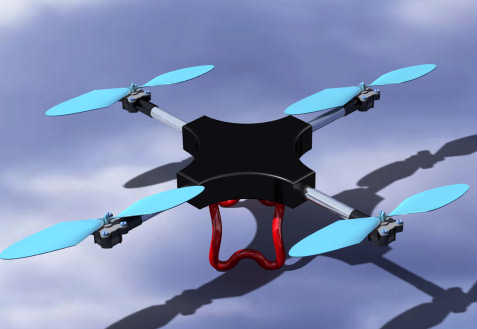
\includegraphics[width=0.5\textwidth]{images/drone_apercu.png}
        \end{center}
        
        \vspace{1.5cm}
        
        \begin{tabular}{l l}
            \textbf{Année académique:} & 2024-2025 \\
        \end{tabular}
        
        \vfill
        
        \begin{tabular}{l l l}
            \textbf{Réalisé par:} & ELARFAOUI Radouan & N° 24 \\
            & HOURIYA & N° 25 \\
        \end{tabular}
        
        \vspace{0.8cm}
        
        \begin{tabular}{l l}
            \textbf{Sous la supervision de:} & [Nom du Professeur] \\
        \end{tabular}
        
        \vspace{1.5cm}
        
        \begin{center}
            \textcolor{bleuPrimaire}{\rule{0.7\textwidth}{1pt}}
        \end{center}
        
        \vspace{0.5cm}
        
        {\Large{\textcolor{gris}{\today}}}
        
    \end{center}
\end{titlepage}

\tableofcontents
\newpage

\chapter{Introduction}

\section{Présentation du projet}
Ce rapport présente le travail réalisé dans le cadre du projet de conception utilisant le logiciel CATIA V5. L'objectif était de concevoir un drone quadrirotor complet, incluant sa structure mécanique et ses systèmes de propulsion.

\section{Contexte et objectifs}
Les drones quadrirotors sont des aéronefs à décollage et atterrissage verticaux (VTOL) qui connaissent un développement considérable ces dernières années. Ils sont utilisés dans de nombreux domaines comme la photographie aérienne, l'inspection de structures, la surveillance, la recherche scientifique ou les loisirs.

Notre projet s'inscrit dans le cadre d'une formation en ingénierie mécanique et vise plusieurs objectifs:
\begin{itemize}
    \item Conception d'un drone quadrirotor fonctionnel et réaliste
    \item Application des principes de conception mécanique
    \item Maîtrise des outils de CAO avancés de CATIA V5
    \item Respect des contraintes de fabrication industrielle
    \item Optimisation des performances (légèreté, rigidité, aérodynamique)
\end{itemize}

\section{Avantages de l'utilisation des drones}
L'utilisation des drones présente de nombreux avantages dans des domaines variés, ce qui en fait une technologie de plus en plus prisée. Ils permettent avant tout d'accéder à des zones difficiles ou dangereuses pour l'homme, comme les sites sinistrés, les hauteurs ou les terrains accidentés, facilitant ainsi les opérations de secours, d'inspection ou de surveillance. En agriculture, les drones sont utilisés pour surveiller les cultures, analyser les sols ou pulvériser avec précision, ce qui améliore les rendements tout en réduisant l'usage de produits. Dans le domaine de la sécurité, ils assurent une surveillance rapide et en temps réel de grands espaces (manifestations, frontières, incendies). Ils sont aussi très utiles dans les médias, pour capturer des images aériennes spectaculaires lors de tournages ou d'événements sportifs. Enfin, leur usage dans la logistique, comme les livraisons rapides de colis ou de médicaments, ouvre la voie à une nouvelle ère de distribution plus réactive, notamment dans les zones isolées. En résumé, les drones permettent de gagner en efficacité, en sécurité et en précision, tout en réduisant souvent les coûts et les risques humains.

\begin{figure}[H]
    \centering
    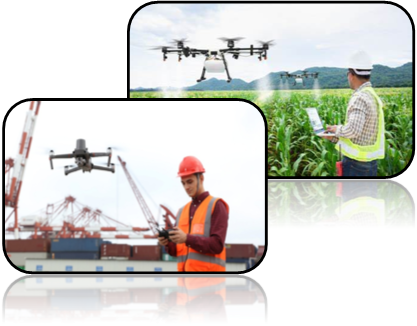
\includegraphics[width=0.7\textwidth]{images/avantages_drones.png}
    \caption{Exemples d'utilisation des drones dans l'agriculture et l'industrie.}
    \label{fig:avantages_drones}
\end{figure}

\section{Analyse fonctionnelle du drone}
L'analyse fonctionnelle permet de définir les besoins auxquels le drone doit répondre, en identifiant ses fonctions principales, contraintes et relations avec l'environnement. Cette démarche est essentielle pour garantir que la conception réponde aux attentes des utilisateurs et aux exigences du cahier des charges.

\subsection{Bête à cornes}
La bête à cornes permet de visualiser le besoin fondamental auquel répond le drone :

\begin{itemize}
    \item \textbf{Qui utilise le drone ?} \quad Utilisateur (opérateur, client)
    \item \textbf{Sur quoi agit-il ?} \quad L'environnement (air, sol, objets à observer ou transporter)
    \item \textbf{Dans quel but ?} \quad Réaliser des missions de prise de vue, de surveillance, de transport léger, etc.
\end{itemize}

\begin{figure}[H]
    \centering
    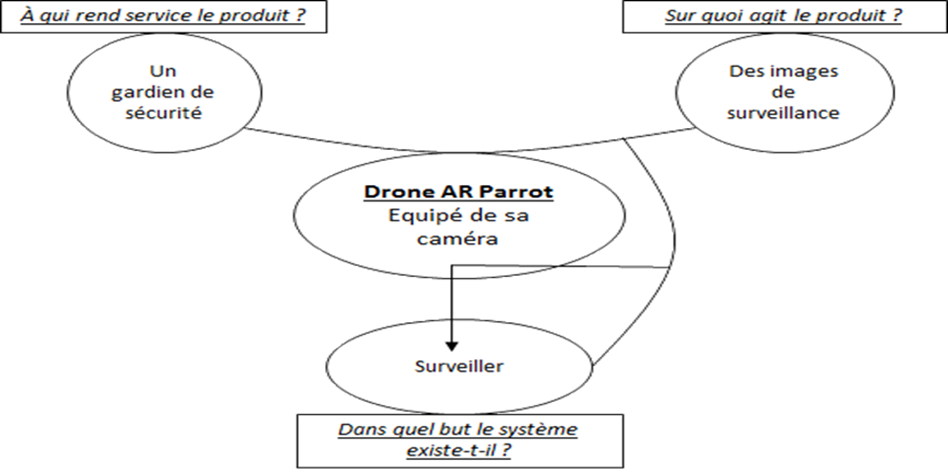
\includegraphics[width=0.7\textwidth]{images/bete_a_corne_surveillance.png}
    \caption{Exemple de bête à cornes pour un drone de surveillance : le drone rend service à un gardien de sécurité, agit sur des images de surveillance, et a pour but de surveiller.}
    \label{fig:bete_a_corne_surveillance}
\end{figure}

\subsection{Diagramme pieuvre}
Le diagramme pieuvre ci-dessous illustre les principales interactions fonctionnelles d'un drone de surveillance avec son environnement. On y retrouve les acteurs, les flux d'information (images de surveillance), l'alimentation (batterie) et les contraintes (conditions climatiques).

\begin{figure}[H]
    \centering
    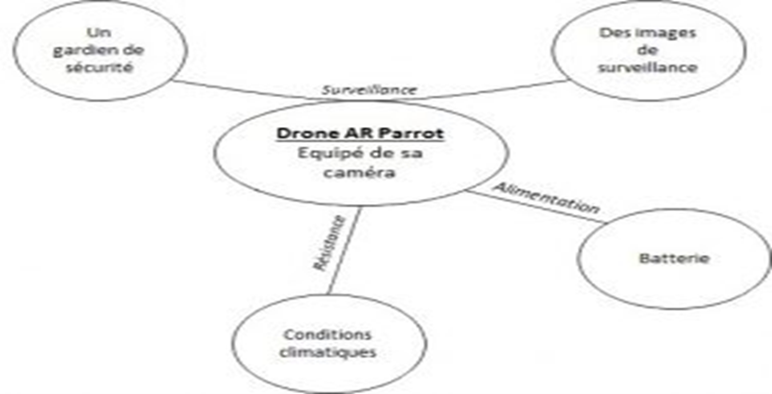
\includegraphics[width=0.7\textwidth]{images/diagramme_pieuvre_surveillance.png}
    \caption{Exemple de diagramme pieuvre pour un drone de surveillance : ce schéma met en évidence les interactions principales du drone avec son environnement.}
    \label{fig:diagramme_pieuvre_surveillance}
\end{figure}

\subsection{Diagramme FAST}
Le diagramme FAST (Function Analysis System Technique) permet de décomposer les fonctions du drone en arborescence, des fonctions principales aux solutions techniques.

\begin{itemize}
    \item \textbf{FP1 : Se déplacer dans l'espace aérien} (fonction principale)
    \item \textbf{FP2 : Transporter une charge utile} (caméra, capteur, petit colis)
    \item \textbf{FP3 : Transmettre des informations} (vidéo, données de capteurs)
    \item \textbf{FC1 : Être alimenté électriquement} (batterie, gestion de l'énergie)
    \item \textbf{FC2 : Être piloté à distance} (télécommande, interface utilisateur)
    \item \textbf{FC3 : Assurer la sécurité des personnes et des biens} (protection, arrêt d'urgence)
    \item \textbf{FC4 : Résister aux conditions extérieures} (vent, pluie, chocs)
\end{itemize}

\begin{figure}[H]
    \centering
    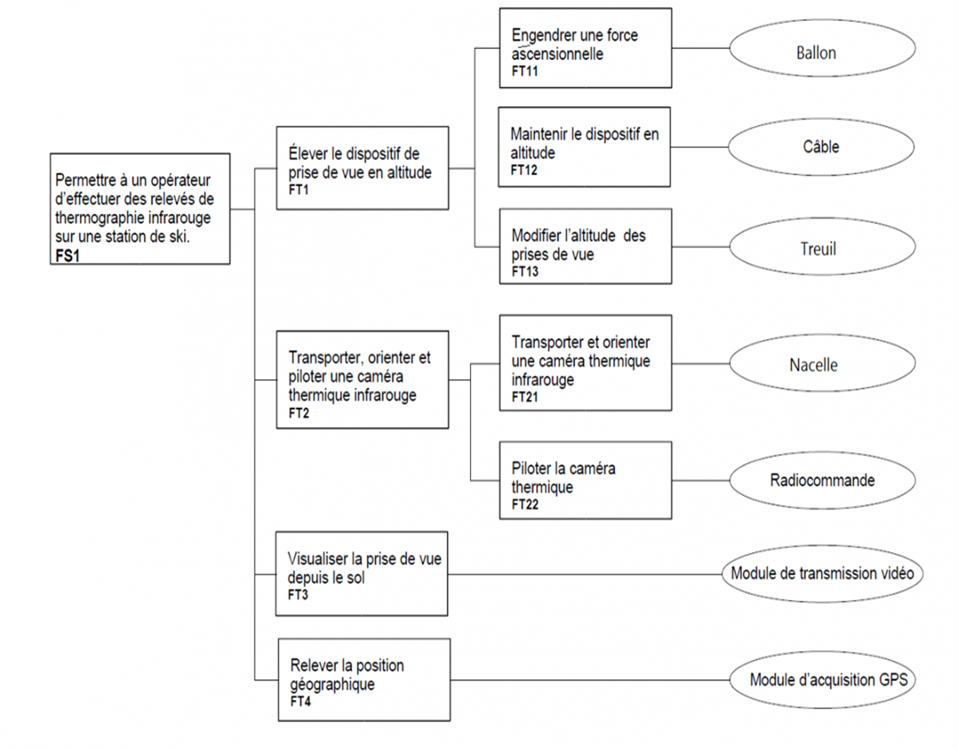
\includegraphics[width=0.9\textwidth]{images/diagramme_fast_exemple.png}
    \caption{Exemple de diagramme FAST : décomposition fonctionnelle d'un système de prise de vue aérienne pour la thermographie infrarouge.}
    \label{fig:diagramme_fast_exemple}
\end{figure}

\subsection{Contraintes}
\begin{itemize}
    \item \textbf{Réglementation} : Respecter les normes de sécurité et d'usage des drones civils
    \item \textbf{Poids} : Limiter la masse pour optimiser l'autonomie
    \item \textbf{Autonomie} : Assurer un temps de vol suffisant pour la mission
    \item \textbf{Robustesse} : Résister aux chocs et aux vibrations
    \item \textbf{Facilité d'utilisation} : Prise en main intuitive, maintenance aisée
    \item \textbf{Coût} : Rester dans un budget raisonnable
\end{itemize}

\section{Cahier des charges}
Le drone devait répondre aux spécifications suivantes:
\begin{itemize}
    \item \textbf{Dimensions}: Envergure maximale de 400mm (entre axes des moteurs opposés)
    \item \textbf{Masse}: Masse totale n'excédant pas 500g (structure seule)
    \item \textbf{Propulsion}: Quatre moteurs brushless avec hélices de 120mm de diamètre
    \item \textbf{Structure}: Résistante aux vibrations et aux contraintes de vol
    \item \textbf{Ergonomie}: Système de prise en main ergonomique
    \item \textbf{Modularité}: Possibilité d'ajouter des accessoires (caméra, capteurs)
    \item \textbf{Fabrication}: Conception compatible avec les procédés d'injection plastique et d'usinage CNC
\end{itemize}

\section{Les composantes du drone}
Un drone est constitué de plusieurs éléments mécaniques, électroniques et logiciels qui travaillent ensemble pour le faire voler, le stabiliser et exécuter des tâches.

\begin{figure}[H]
    \centering
    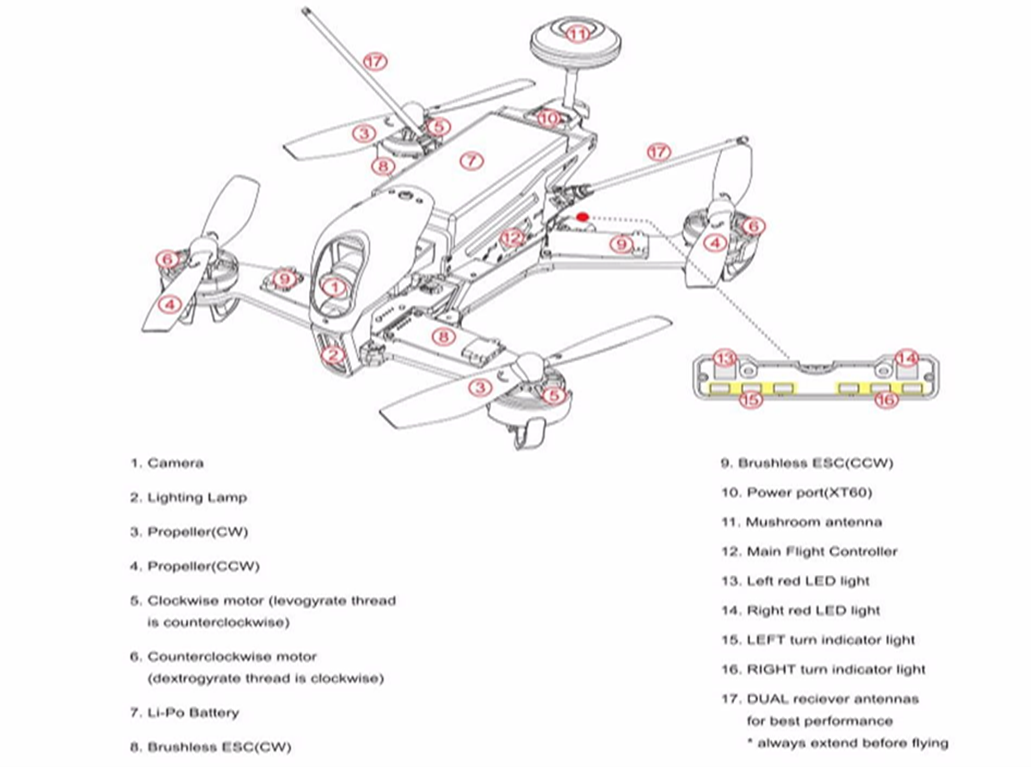
\includegraphics[width=0.95\textwidth]{images/composantes_drone_exemple.png}
    \caption{Exemple de répartition des principales composantes d'un drone moderne (source : manuel constructeur).}
    \label{fig:composantes_drone_exemple}
\end{figure}

\section{Schéma cinématique et fonctionnement}

L'étude du drone s'intéresse essentiellement à la partie du corps principal, comme le montre la figure ci-dessous :

\begin{figure}[H]
    \centering
    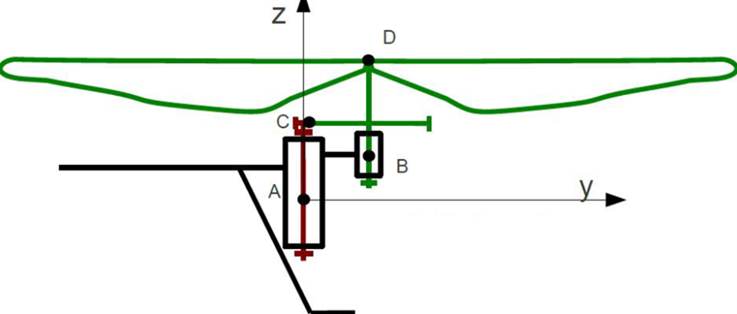
\includegraphics[width=0.8\textwidth]{images/schema_cinematique_drone.png}
    \caption{Schéma cinématique d'un drone quadrirotor : axes de commande (gaz, lacet, roulis, tangage).}
    \label{fig:schema_cinematique_drone}
\end{figure}

\subsection*{Rôle des principaux éléments et liaisons cinématiques}

\textbf{Hélices et rotors :} Les hélices sont fixées aux moteurs et forment une liaison pivot. En tournant, elles déplacent l'air et génèrent une portance verticale qui permet au drone de décoller et de manœuvrer. Chaque rotor crée un flux d'air vers le bas, produisant une force vers le haut selon le même principe qu'un hélicoptère.

\begin{figure}[H]
    \centering
    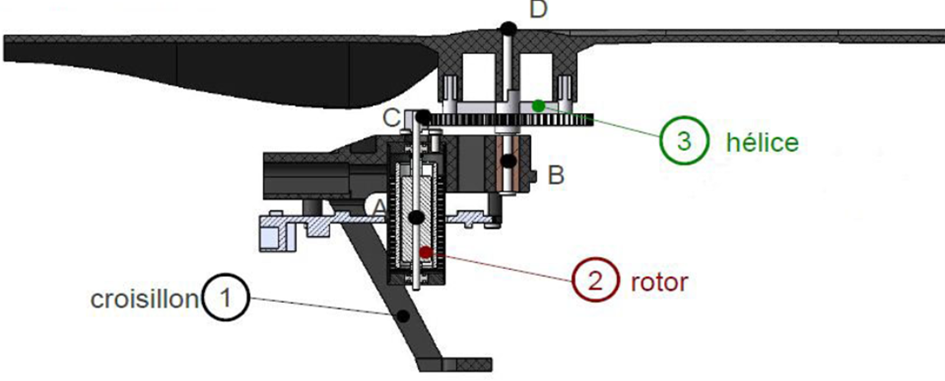
\includegraphics[width=0.9\textwidth]{images/coupe_rotor_croisillon.png}
    \caption{Coupe d'un ensemble rotor-hélice-croisillon d'un drone.}
    \label{fig:coupe_rotor_croisillon}
\end{figure}

\textbf{Croisillon :} Il joue un rôle fondamental dans la structure et la stabilité du drone, reliant les moteurs entre eux dans une configuration équilibrée. La liaison entre les moteurs et le croisillon est fixe (rigide), maintenant les moteurs solidaires de la structure.

\subsection*{Types de liaisons dans l'architecture du drone}
\begin{enumerate}
    \item \textbf{Liaison rigide} entre le croisillon et les moteurs : fixation solide par vis ou écrous.
    \item \textbf{Liaison pivot} pour les rotors : permet aux hélices de tourner autour de leur axe.
    \item \textbf{Liaison structurelle} entre le croisillon et le corps central : maintient les bras du drone.
    \item \textbf{Liaison amortie} (facultative) : réduit les vibrations entre le croisillon et les composants électroniques.
\end{enumerate}

\subsection*{Principe de fonctionnement}
Le contrôle du drone repose sur la variation différentielle de vitesse des moteurs. Le contrôleur de vol ajuste en temps réel la vitesse de chaque moteur pour :
\begin{itemize}
    \item Contrôler l'altitude (gaz) : variation simultanée de la vitesse des quatre moteurs
    \item Contrôler le roulis et le tangage : variation opposée des paires de moteurs
    \item Contrôler le lacet : variation opposée de la vitesse entre moteurs tournant dans le même sens
\end{itemize}

Ce système intégré combine mécanique, électronique et logiciels pour garantir un vol stable et contrôlé.

\section{Démarche adoptée}
Pour réaliser ce projet, nous avons suivi une méthodologie structurée:
\begin{enumerate}
    \item Étude de l'existant et analyse des solutions techniques
    \item Conception préliminaire des différentes pièces
    \item Validation technique par simulation numérique
    \item Conception détaillée des composants
    \item Assemblage virtuel et vérification des interférences
    \item Réalisation des dessins de définition et d'ensemble
\end{enumerate}

\section{Outils utilisés}
Pour réaliser ce projet, nous avons principalement utilisé CATIA V5, un logiciel de conception assistée par ordinateur (CAO) développé par Dassault Systèmes. Ce logiciel nous a permis de modéliser les différentes pièces, de réaliser les assemblages et de générer les dessins techniques.

\subsection{Modules CATIA utilisés}
Plusieurs modules de CATIA V5 ont été mobilisés pour ce projet:
\begin{itemize}
    \item \textbf{Part Design}: Pour la modélisation 3D des pièces
    \item \textbf{Assembly Design}: Pour l'assemblage des composants
    \item \textbf{Drafting}: Pour la création des dessins techniques
    \item \textbf{DMU Kinematics}: Pour la simulation des mouvements
    \item \textbf{Generative Shape Design}: Pour la création de surfaces complexes (hélices)
\end{itemize}


\begin{figure}[H]
    \centering
    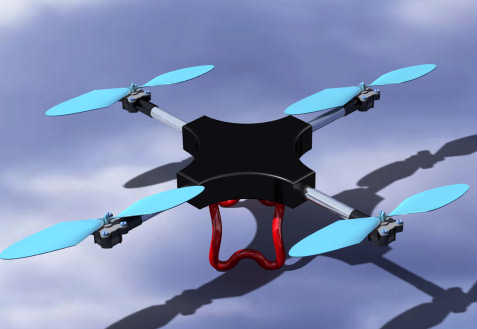
\includegraphics[width=0.8\textwidth]{images/drone_apercu.png}
    \caption{Aperçu du drone quadrirotor conçu dans ce projet}
    \label{fig:drone_apercu}
\end{figure}

Le rapport qui suit détaille l'ensemble du processus de conception, depuis la modélisation des pièces individuelles jusqu'à l'assemblage complet, en passant par les dessins techniques.

\chapter{Conception des pièces}
\section{Liste des pièces modélisées}
Dans ce projet, nous avons modélisé les pièces suivantes:
\begin{itemize}
    \item Pièce 1: Châssis central (corps principal)
    \item Pièce 2: Bras de support des moteurs (4 pièces)
    \item Pièce 3: Supports de moteur (4 pièces, fixés aux extrémités des bras)
    \item Pièce 4: Hélices (4 pièces, de couleur bleue)
    \item Pièce 5: Moteurs brushless (4 pièces)
    \item Pièce 6: Support d'attache (en rouge)
    \item Pièce 7: Éléments de fixation (vis et écrous pour l'assemblage)
    \item Pièce 8: Capot de protection électronique
    % Ajoutez d'autres pièces selon votre projet
\end{itemize}

\section{Procédures de modélisation}
\subsection{Modélisation du châssis central}
Pour modéliser le châssis central du drone, nous avons suivi les étapes suivantes:
\begin{enumerate}
    \item \textbf{Création d'une esquisse sur le plan XY}:
    \begin{itemize}
        \item Dessin d'un octogone régulier comme base du châssis
        \item Application des contraintes de symétrie par rapport aux axes
        \item Cotation du diamètre extérieur à 160mm
    \end{itemize}
    
    \begin{figure}[H]
        \centering
        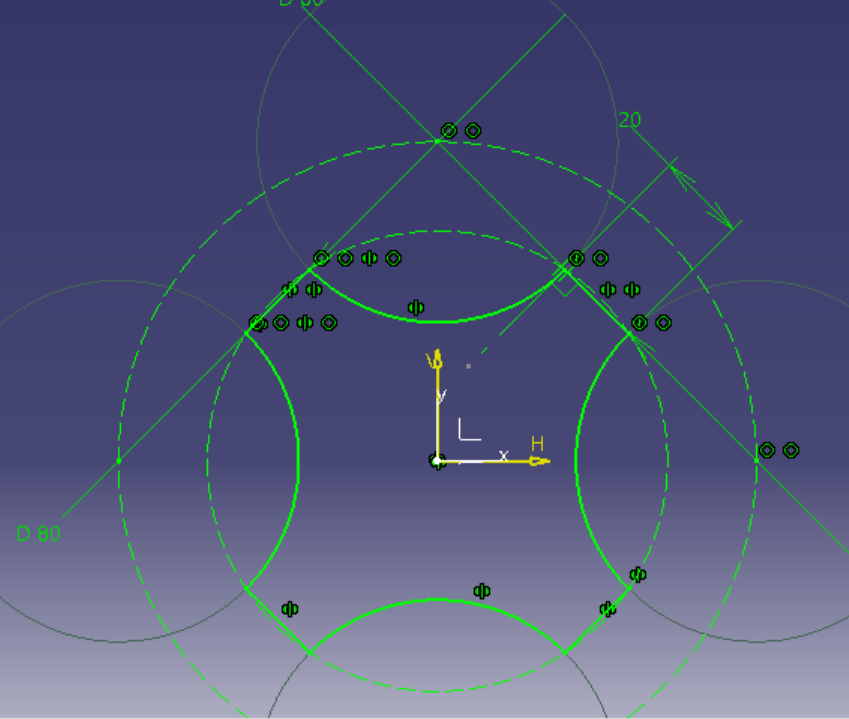
\includegraphics[width=0.8\textwidth]{images/esquisse_chassis_central.png}
        \caption{Extrait du dessin de définition du châssis central}
        \label{fig:dessin_def}
    \end{figure}
    
    \item \textbf{Extrusion (Pad) de l'esquisse}:
    \begin{itemize}
        \item Extrusion de 20mm dans la direction Z positif
    \end{itemize}
    
    \begin{figure}[H]
        \centering
        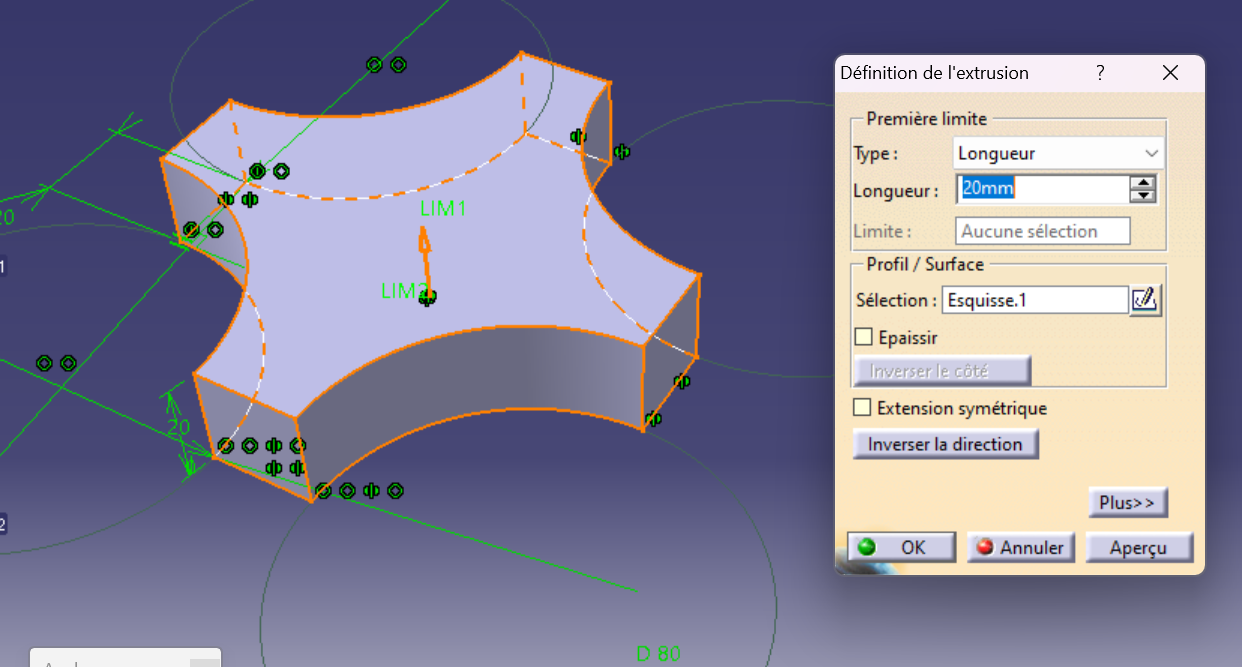
\includegraphics[width=0.8\textwidth]{images/extrusion_chassis_central.png}
        \caption{Opération d'extrusion (Pad) du châssis central de 20mm}
        \label{fig:extrusion_chassis}
    \end{figure}
    
    \item \textbf{Création d'un trou taraudé}:
    \begin{itemize}
        \item Définition d'un trou taraudé M8 sur la face avant du châssis
        \item Profondeur du trou: 10mm
        \item Type de taraudage: Métrique à pas épais
        \item Diamètre avant trou: M8 (7mm)
        \item Profondeur du taraudage: 10mm 
    \end{itemize}
    
    \begin{figure}[H]
        \centering
        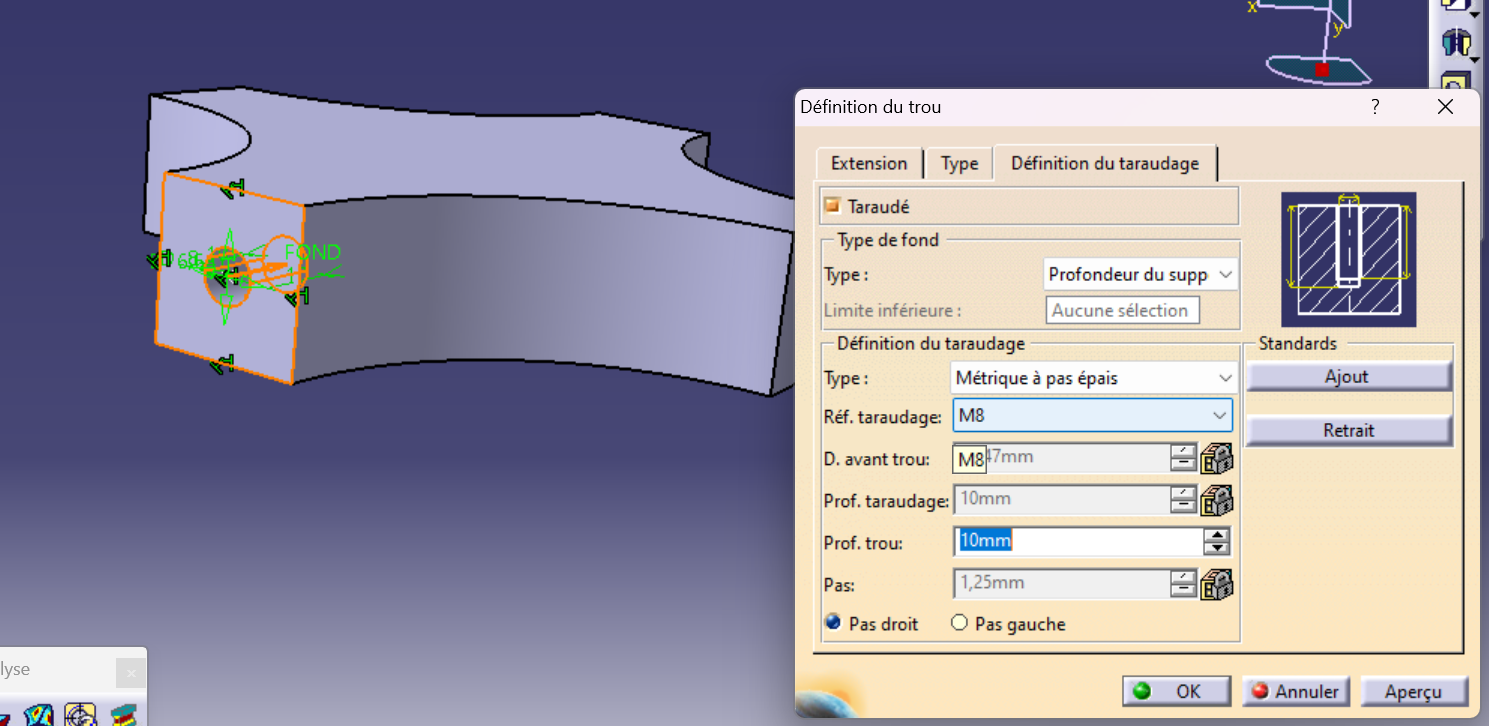
\includegraphics[width=0.8\textwidth]{images/trou_taraude_chassis.png}
        \caption{Création d'un trou taraudé M8 dans le châssis central}
        \label{fig:trou_taraude}
    \end{figure}
    
    \item \textbf{Création d'une répétition circulaire}:
    \begin{itemize}
        \item Application d'un pattern circulaire (Circular Pattern) du trou taraudé
        \item Nombre d'instances: 4
        \item Espacement angulaire: 90 degrés (360° divisé en 4 instances)
        \item Référence axiale: axe central du châssis
        \item Composant à copier: trou.1 
    \end{itemize}
    
    \begin{figure}[H]
        \centering
        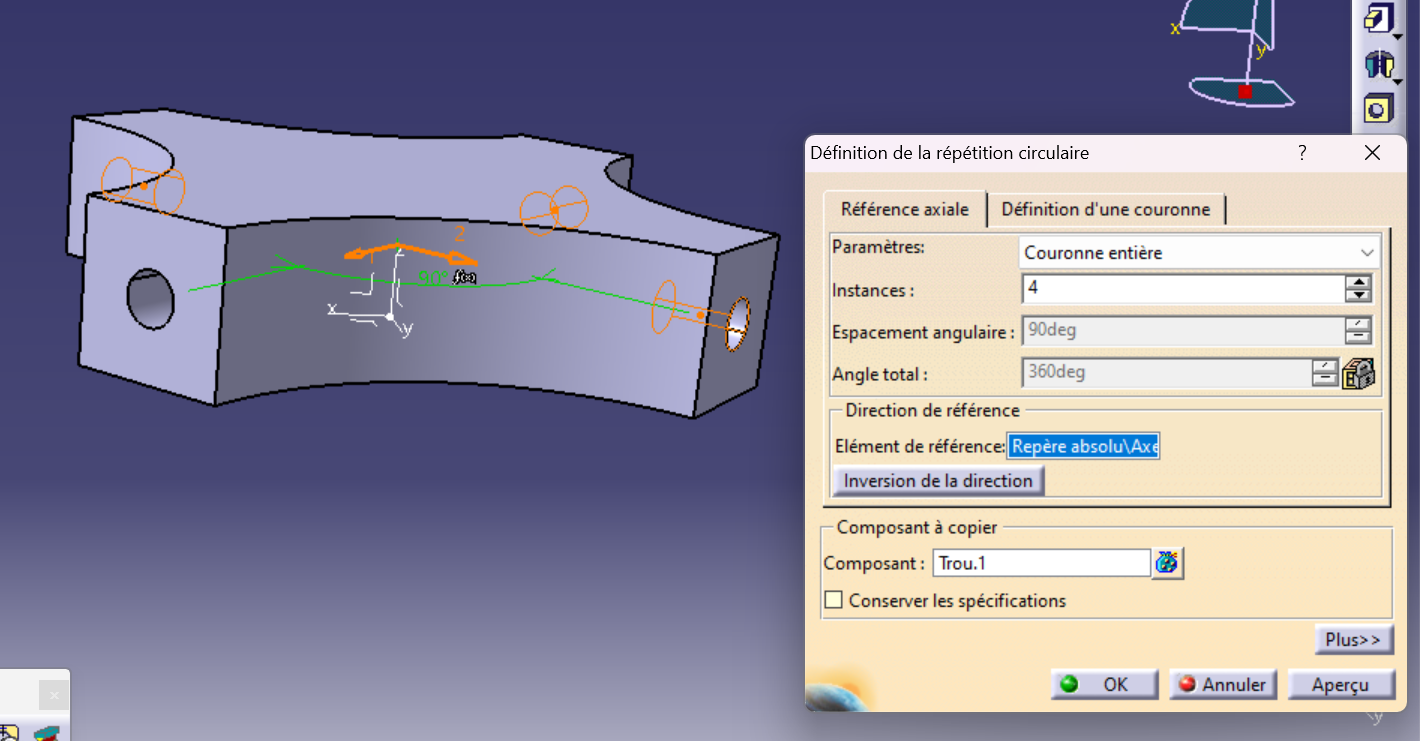
\includegraphics[width=0.8\textwidth]{images/repetition_circulaire_trou.png}
        \caption{Répétition circulaire des trous taraudés M8 à 90° d'intervalle}
        \label{fig:repetition_circulaire}
    \end{figure}
    
    \item \textbf{Application de congés}:
    \begin{itemize}
        \item Utilisation de la fonction Congé (Fillet) pour adoucir les arêtes
        \item Rayon du congé: 2mm
        \item Sélection des arêtes extérieures du châssis (2 éléments)
        \item Mode de sélection: Tangence
    \end{itemize}
    
    \begin{figure}[H]
        \centering
        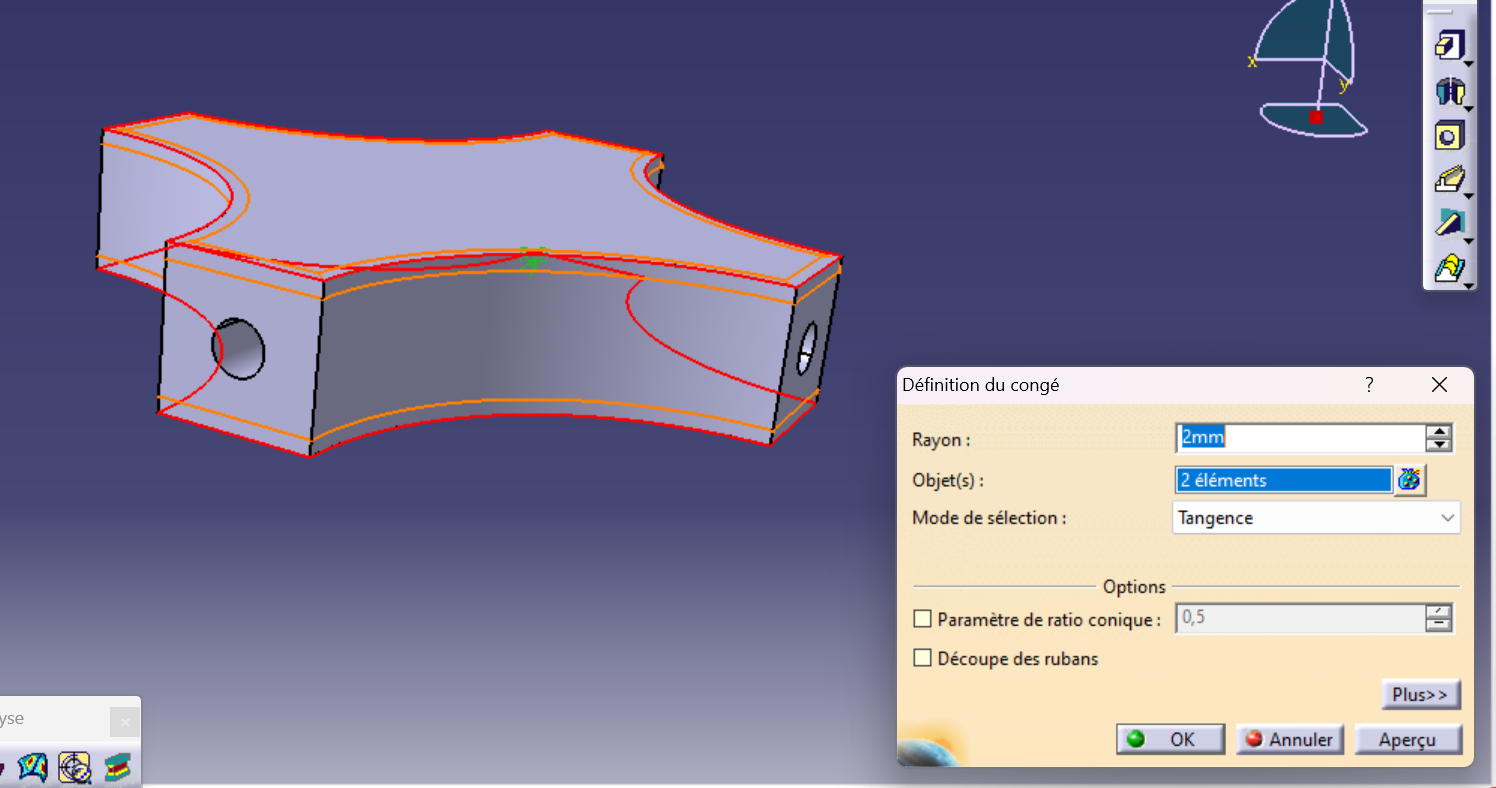
\includegraphics[width=0.8\textwidth]{images/conge_chassis.png}
        \caption{Application de congés de rayon 2mm sur les arêtes du châssis}
        \label{fig:conge_chassis}
    \end{figure}
    
    \item \textbf{Création de poches pour la fixation des pieds}:
    \begin{itemize}
        \item Création d'une nouvelle esquisse (Esquisse.4) sur la face supérieure du châssis
        \item Dessin des contours pour les emplacements des fixations des pieds
        \item Utilisation de la fonction Poche (Pocket) pour creuser ces emplacements
        \item Profondeur de la poche: 6mm
        \item Type: Longueur (type de limite standard)
    \end{itemize}
    
    \begin{figure}[H]
        \centering
        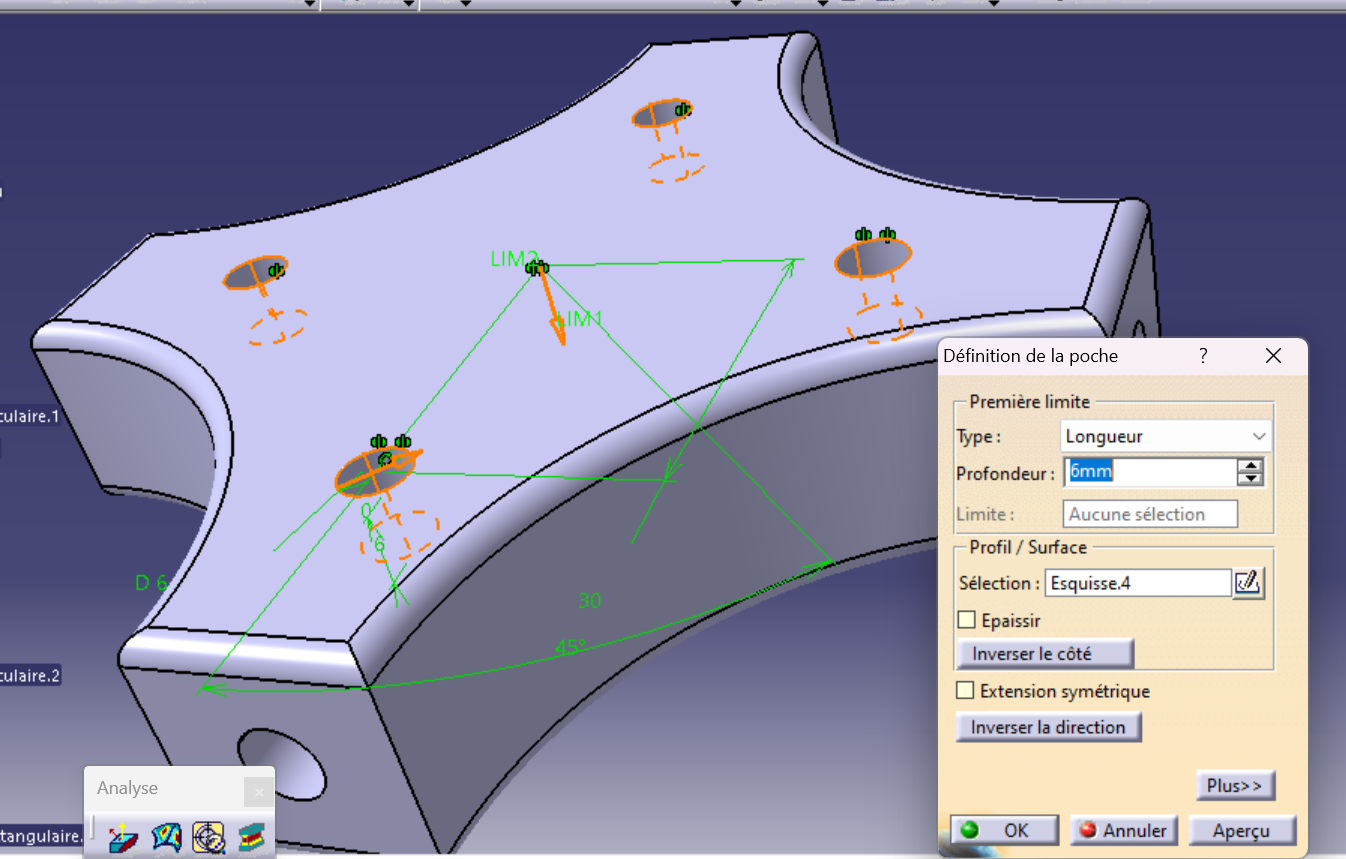
\includegraphics[width=0.8\textwidth]{images/poche_fixation_pieds.png}
        \caption{Création des poches pour la fixation des pieds du drone}
        \label{fig:poche_pieds}
    \end{figure}
    
    \item \textbf{Création de la poche centrale pour l'électronique}:
    \begin{itemize}
        \item Création d'une nouvelle esquisse (Esquisse.5) au centre du châssis
        \item Dessin d'une forme ovale/elliptique pour optimiser l'espace disponible
        \item Utilisation de la fonction Poche (Pocket) pour créer le logement des composants
        \item Type de limite: Jusqu'au suivant
        \item Décalage: -4mm pour laisser une épaisseur suffisante au fond du châssis
    \end{itemize}
    
    \begin{figure}[H]
        \centering
        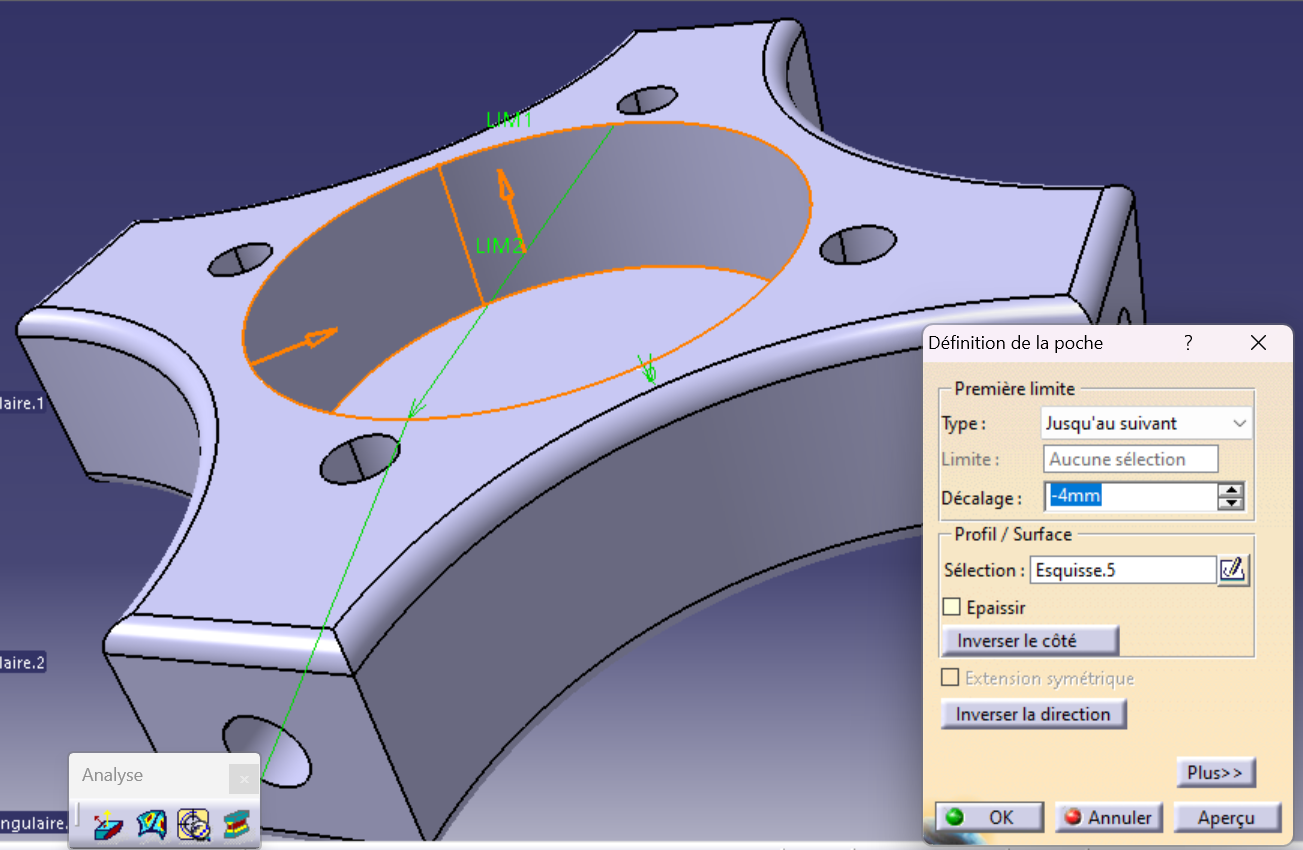
\includegraphics[width=0.8\textwidth]{images/poche_electronique.png}
        \caption{Création de la poche centrale pour les composants électroniques et de contrôle}
        \label{fig:poche_electronique}
    \end{figure}
    
    \item \textbf{Création des nervures de renforcement}:
    \begin{itemize}
        \item Création d'une nouvelle esquisse (Esquisse.6) sur la face inférieure de la poche centrale
        \item Dessin d'un motif de nervures parallèles pour le renforcement structurel
        \item Utilisation de la fonction Extrusion (Rib/Nervure) pour créer les éléments de renfort
        \item Première limite: Type "Jusqu'au suivant" avec décalage de 0mm
        \item Seconde limite: Type "Longueur" avec valeur -14mm (vers le bas)
        \item Épaississement de 1mm pour les nervures
        \item Option "Perpendiculaire au contour" sélectionnée
    \end{itemize}
    
    \begin{figure}[H]
        \centering
        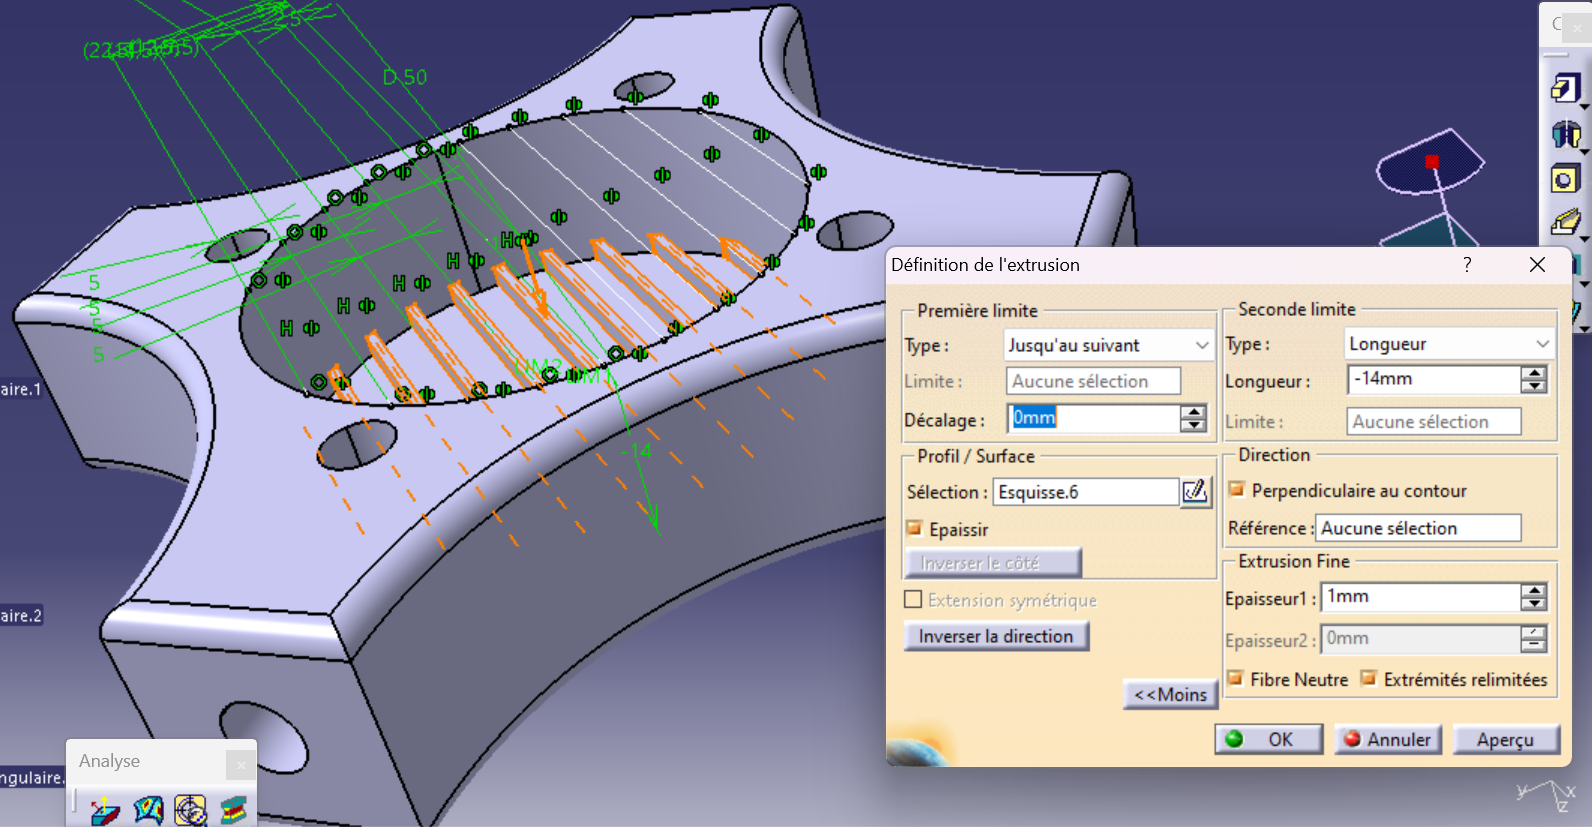
\includegraphics[width=0.8\textwidth]{images/nervures_renforcement.png}
        \caption{Création des nervures de renforcement par extrusion}
        \label{fig:nervures_renforcement}
    \end{figure}
    
    \item \textbf{Répétition circulaire des nervures}:
    \begin{itemize}
        \item Application d'un pattern circulaire (Circular Pattern) aux nervures de renforcement
        \item Composant à copier: Extrusion.2 (ensemble des nervures initiales)
        \item Nombre d'instances: 2
        \item Espacement angulaire: 90 degrés
        \item Angle total: 90 degrés (pour une disposition orthogonale)
        \item Élément de référence: Repère absolu/Axe
        \item Création d'un motif en quadrillage pour un renforcement optimal
    \end{itemize}
    
    \begin{figure}[H]
        \centering
        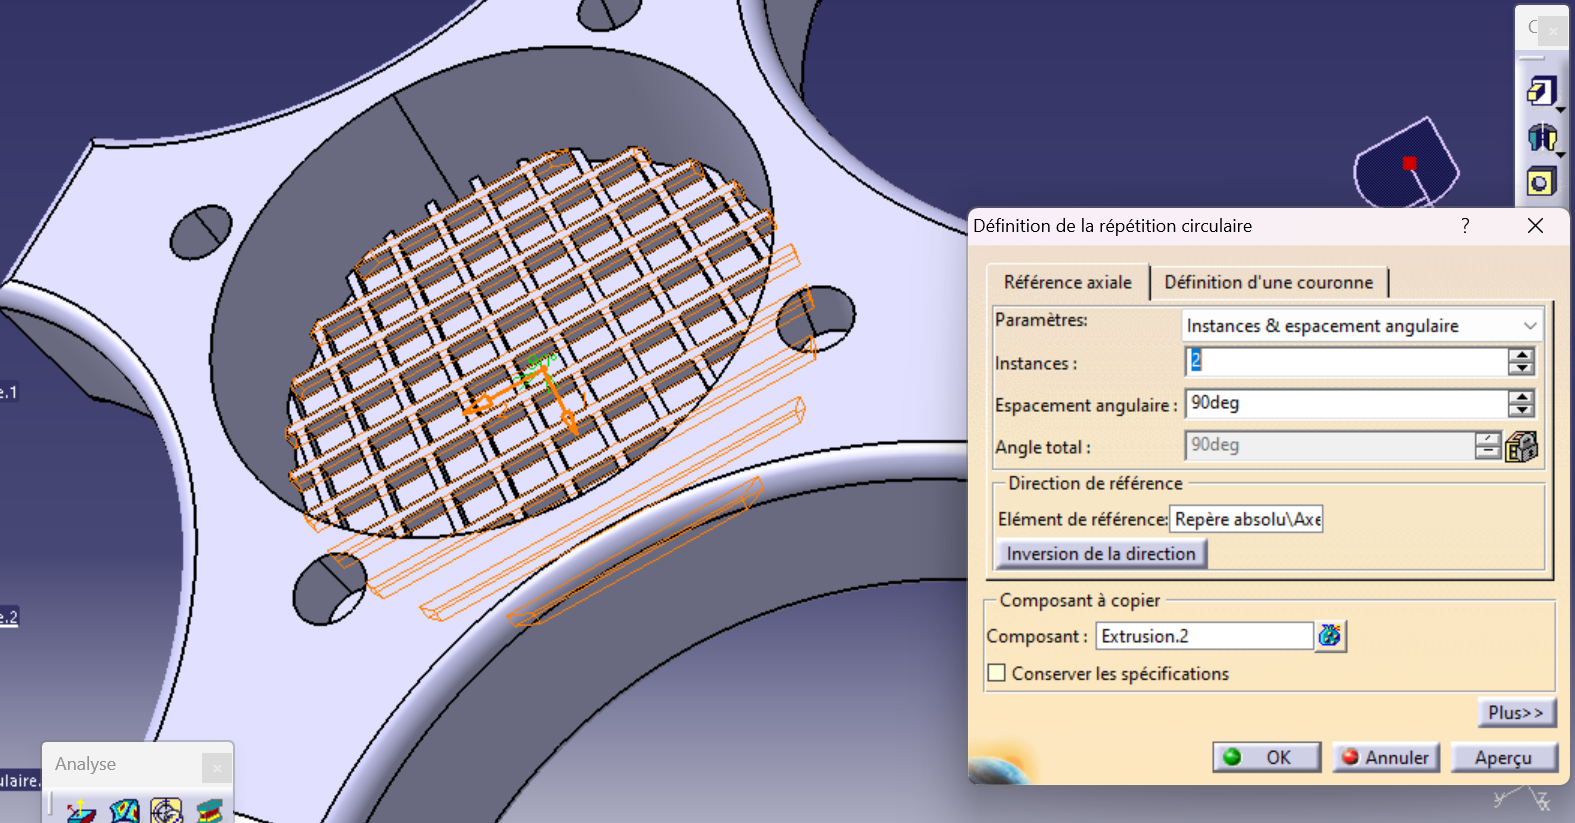
\includegraphics[width=0.8\textwidth]{images/repetition_nervures.png}
        \caption{Répétition circulaire des nervures formant un quadrillage de renforcement}
        \label{fig:repetition_nervures}
    \end{figure}
    
    \item \textbf{Création des supports de fixation pour le couvercle}:
    \begin{itemize}
        \item Création d'une nouvelle esquisse (Esquisse.7) à l'intersection des nervures
        \item Utilisation de la fonction Extrusion (Pad/Extrusion) pour créer les piliers de fixation
        \item Première limite: Type "Jusqu'au plan" avec la face de la poche comme référence
        \item Seconde limite: Type "Jusqu'au plan" avec décalage de 1mm
        \item Utilisation d'un profil rectangulaire aux intersections des nervures
        \item Ces supports recevront ultérieurement un taraudage pour la fixation du couvercle
    \end{itemize}
    
    \begin{figure}[H]
        \centering
        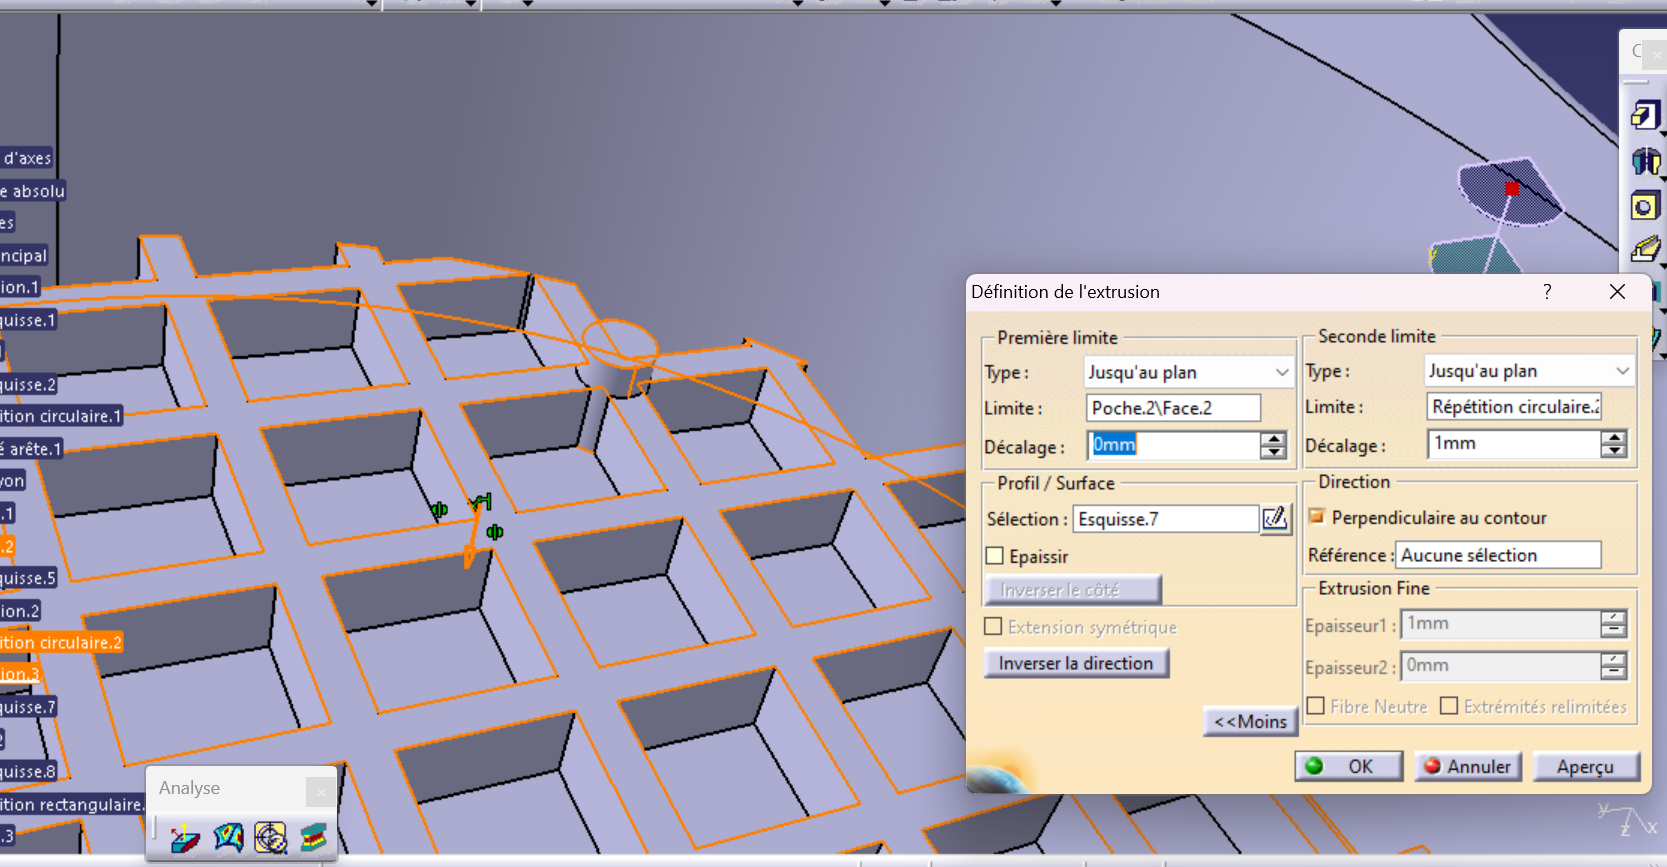
\includegraphics[width=0.8\textwidth]{images/supports_fixation_couvercle.png}
        \caption{Création des supports pour la fixation du couvercle au châssis}
        \label{fig:supports_fixation}
    \end{figure}
    
    \item \textbf{Création des taraudages pour le couvercle}:
    \begin{itemize}
        \item Utilisation de la fonction Trou (Hole) avec l'option Taraudé
        \item Type de taraudage: Métrique à pas épais
        \item Référence de taraudage: M1.6
        \item Diamètre avant trou: 1,221mm
        \item Profondeur de taraudage: 6mm
        \item Profondeur de trou: 6mm
        \item Pas: 0,35mm
        \item Option "Pas droit" sélectionnée
        \item Ces taraudages permettront de fixer solidement le couvercle protégeant l'électronique
    \end{itemize}
    
    \begin{figure}[H]
        \centering
        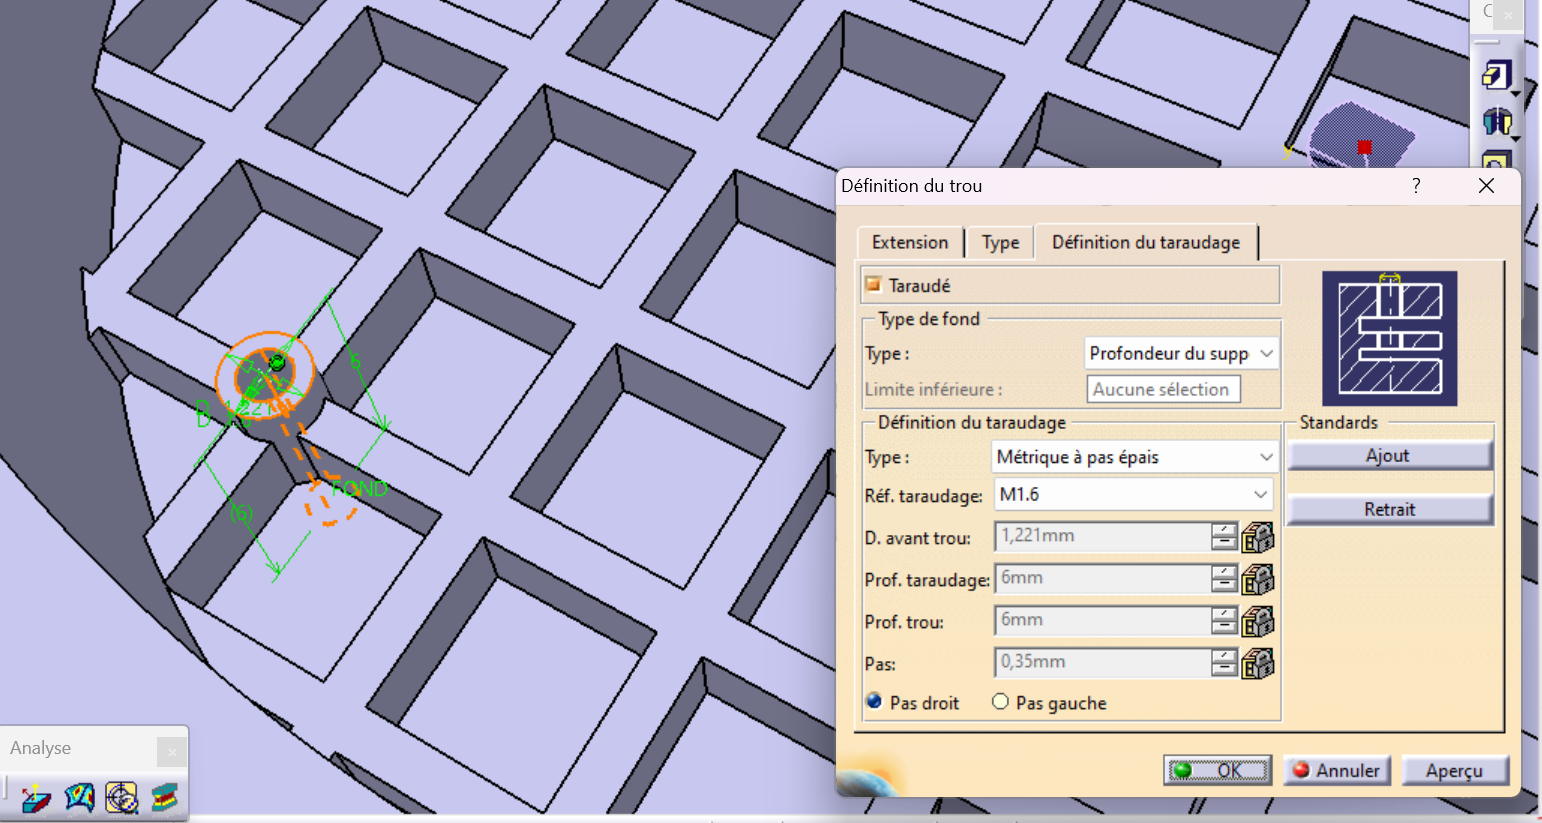
\includegraphics[width=0.8\textwidth]{images/taraudage_couvercle.png}
        \caption{Création des taraudages M1.6 pour la fixation du couvercle}
        \label{fig:taraudage_couvercle}
    \end{figure}
    
    \item \textbf{Répétition rectangulaire des taraudages}:
    \begin{itemize}
        \item Application d'un pattern rectangulaire (Rectangular Pattern) aux taraudages
        \item Composant à copier: Trou.2 (taraudage M1.6 initial)
        \item Paramètres: Instances \& espacement
        \item Première direction: 2 instances avec un espacement de 25mm
        \item Longueur totale: 25mm
        \item Élément de référence: Repère absolu/Axe
        \item Cette répétition crée un ensemble de taraudages uniformément répartis
        \item Les points de fixation aux quatre coins garantissent une fermeture stable du couvercle
    \end{itemize}
    
    \begin{figure}[H]
        \centering
        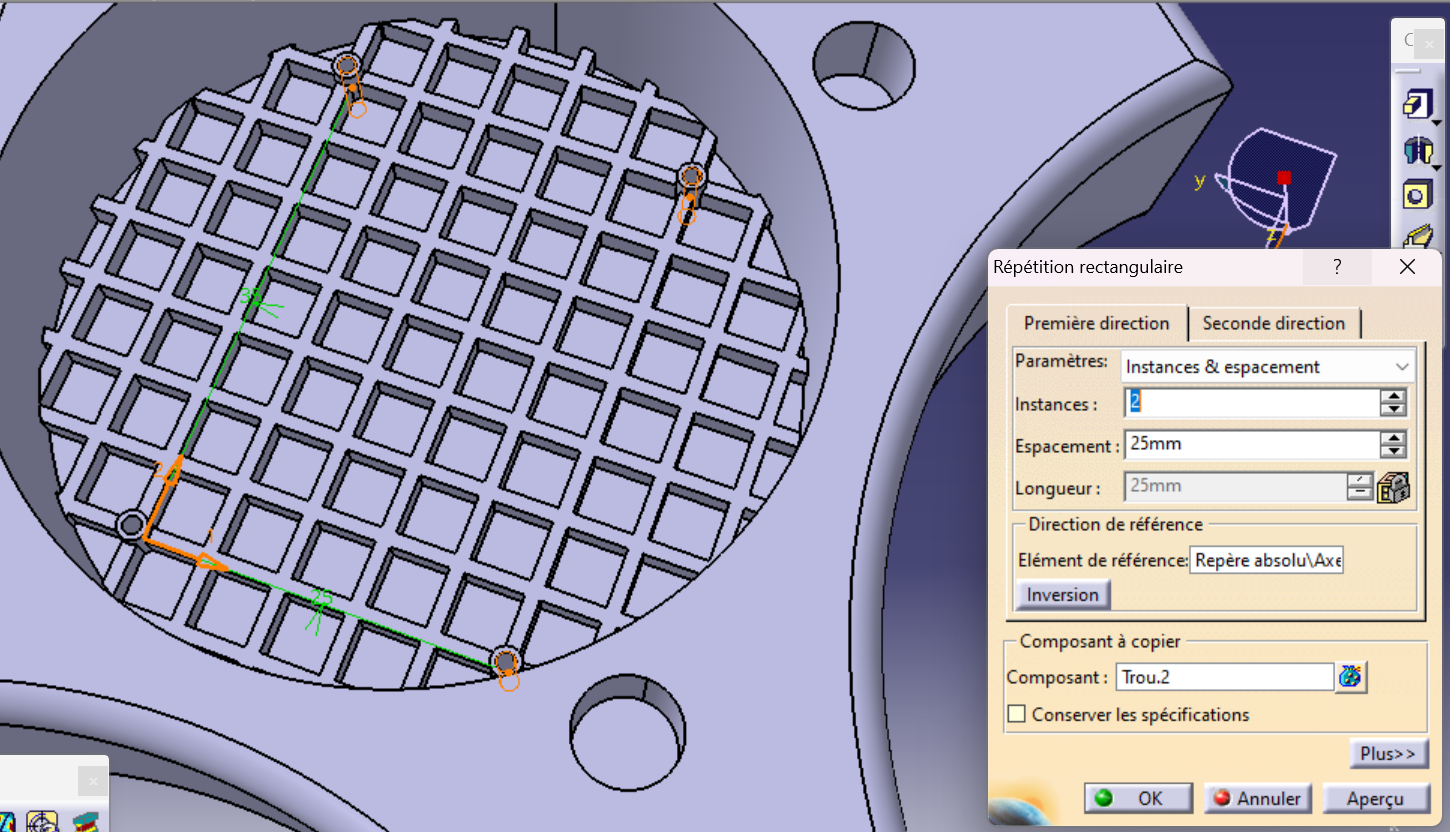
\includegraphics[width=0.8\textwidth]{images/repetition_taraudages.png}
        \caption{Répétition rectangulaire des taraudages pour la fixation du couvercle}
        \label{fig:repetition_taraudages}
    \end{figure}
    
    \item \textbf{Création du logement pour le centrage du couvercle}:
    \begin{itemize}
        \item Création d'une nouvelle esquisse (Esquisse.10) sur la face supérieure du châssis
        \item Dessin d'un cercle concentrique définissant le contour du couvercle
        \item Utilisation de la fonction Poche (Pocket) pour créer un léger rebord
        \item Profondeur de la poche: 2mm
        \item Type: Longueur (type de limite standard)
        \item Ce rebord circulaire servira à positionner et centrer précisément le couvercle
        \item Il permettra également d'assurer l'étanchéité de la zone des composants électroniques
    \end{itemize}
    
    \begin{figure}[H]
        \centering
        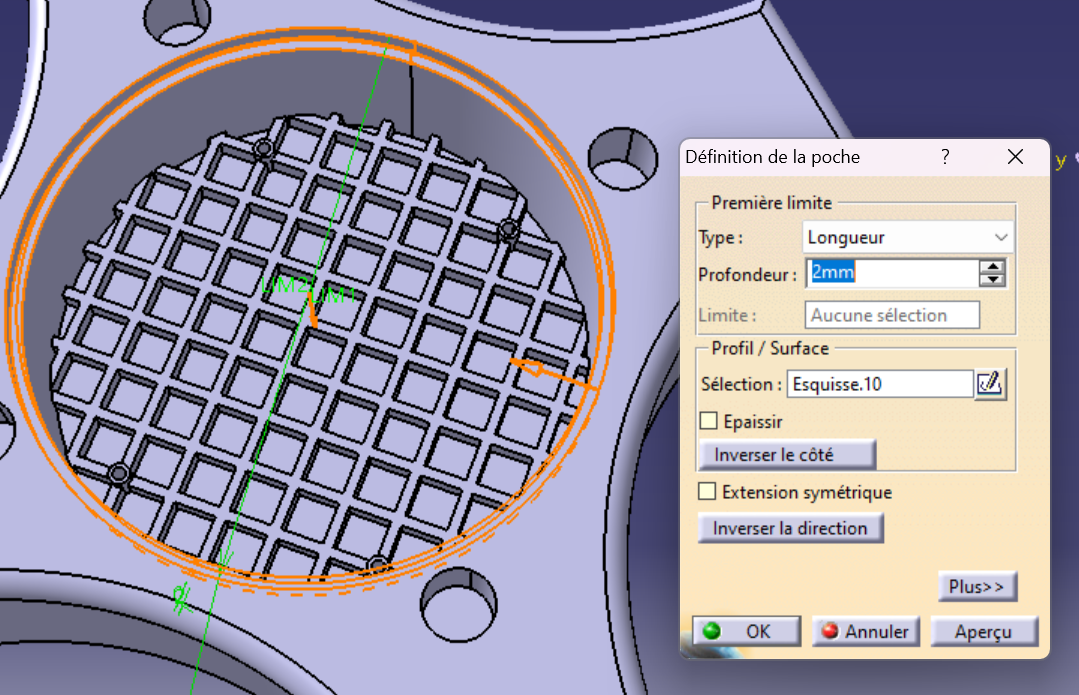
\includegraphics[width=0.8\textwidth]{images/logement_couvercle.png}
        \caption{Création du logement circulaire pour le centrage du couvercle de protection}
        \label{fig:logement_couvercle}
    \end{figure}
    
    \item \textbf{Finalisation du châssis central}:
    \begin{itemize}
        \item Le châssis central est maintenant terminé avec toutes ses fonctionnalités intégrées
        \item La pièce finale comprend les éléments suivants :
        \begin{itemize}
            \item Un corps principal extrudé de 20mm d'épaisseur
            \item Quatre trous taraudés M8 pour la fixation des bras, disposés à 90° d'intervalle
            \item Des congés de 2mm sur les arêtes extérieures pour améliorer l'ergonomie et la résistance
            \item Des poches pour la fixation des pieds du drone
            \item Une cavité centrale pour loger les composants électroniques
            \item Une structure de renforcement en quadrillage pour optimiser le rapport résistance/poids
            \item Des points de fixation avec taraudages M1.6 pour le couvercle de protection
            \item Un rebord circulaire de 2mm de profondeur pour le centrage précis du couvercle
        \end{itemize}
        \begin{figure}[H]
            \centering
            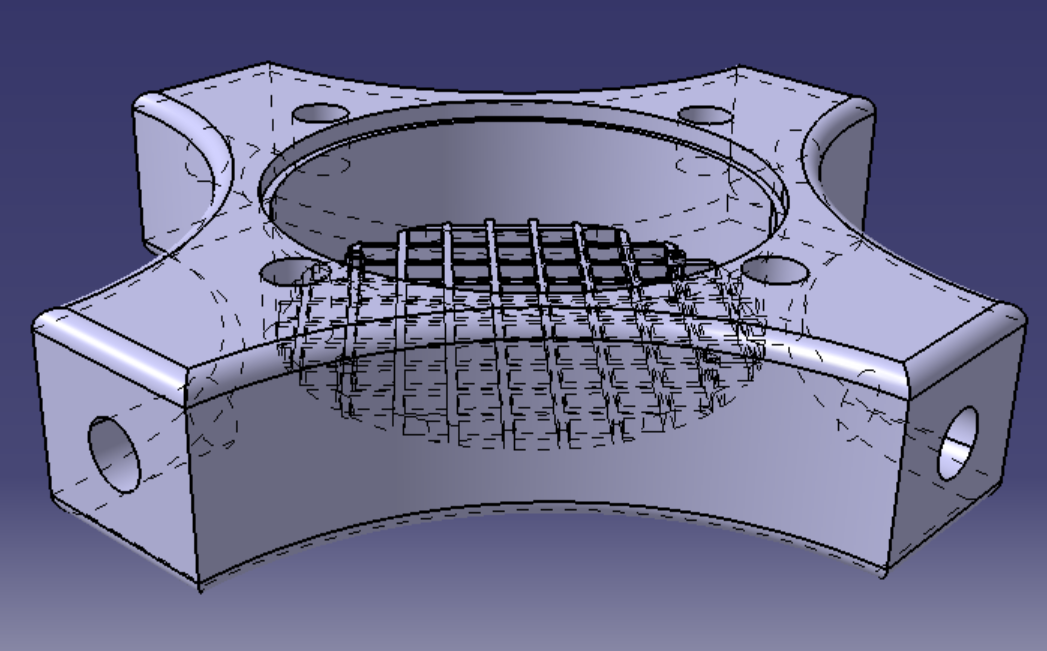
\includegraphics[width=0.7\textwidth]{images/chassis_central_final.png}
            \caption{Châssis central complet}
            \label{fig:chassis_central_complet}
        \end{figure}
        \item Cette pièce centrale constitue le cœur structurel du drone, intégrant harmonieusement les fonctions mécaniques et les considérations d'assemblage
    \end{itemize}
\end{enumerate}

\subsection{Modélisation des bras de support}
Pour modéliser les bras qui supportent les moteurs, nous avons procédé comme suit:
\begin{enumerate}
    \item \textbf{Modélisation du tube de liaison}:
    \begin{itemize}
        \item Création d'une esquisse (Esquisse.2) avec deux cercles concentriques
        \item Cercle extérieur de diamètre 10mm
        \item Cercle intérieur de diamètre 8mm (épaisseur de paroi de 1mm)
        \item Utilisation de la fonction Extrusion (Pad) pour créer le corps cylindrique
        \item Longueur d'extrusion: 30mm avec l'option d'extension symétrique activée
        \item Longueur totale obtenue: 60mm (30mm de chaque côté du plan d'esquisse)
        \item Le profil tubulaire permet un excellent rapport résistance/poids
        \item L'aluminium a été choisi pour sa légèreté et sa bonne résistance mécanique
    \end{itemize}
    \begin{figure}[H]
        \centering
        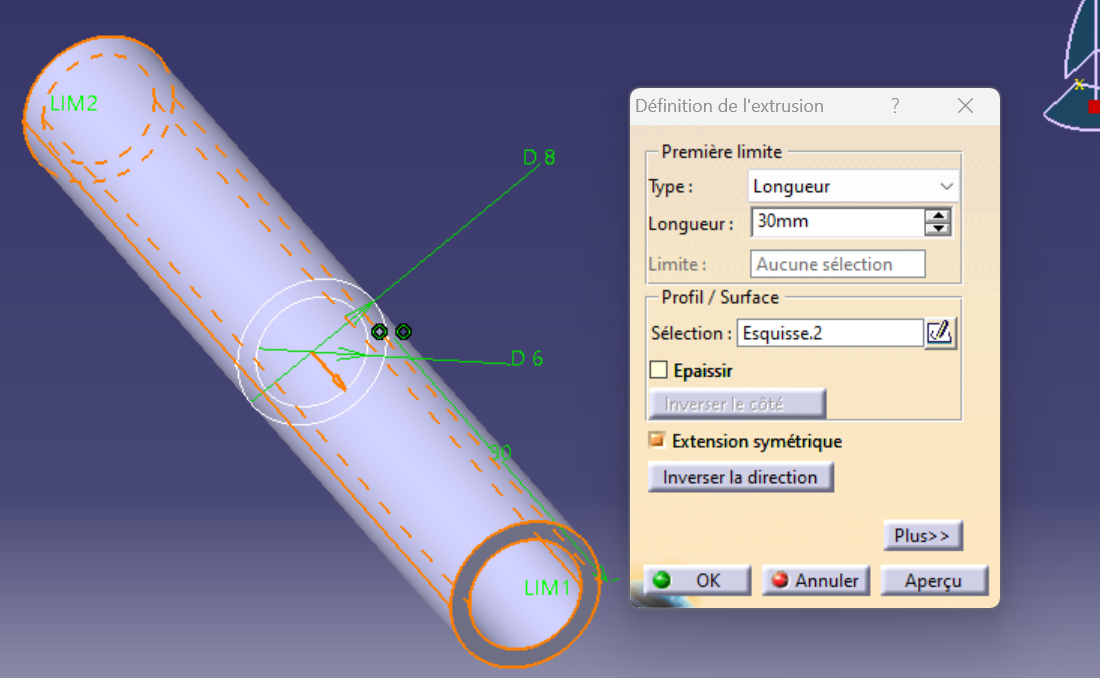
\includegraphics[width=0.7\textwidth]{images/extrusion_tube.png}
        \caption{Extrusion du tube de liaison}
        \label{fig:extrusion_tube}
    \end{figure}
    
    \item \textbf{Création des fixations hélicoïdales}:
    \begin{itemize}
        \item Ajout de filetages aux extrémités du tube pour la fixation
        \item Utilisation de la fonction filetage/taraudage (Thread/Tap) intégrée à CATIA V5
        \item Sélection de l'option "Filetage" (option sélectionnée dans l'interface)
        \item Définition géométrique:
        \begin{itemize}
            \item Face latérale: Taraudage.1/Face.1
            \item Face limite: Taraudage.1/Face.3
        \end{itemize}
        \item Définition numérique du filetage:
        \begin{itemize}
            \item Type: Métrique pas gros
            \item Référence: M8
            \item Diamètre du support: 8mm (diamètre intérieur du tube)
            \item Profondeur de taraudage: 10mm
            \item Hauteur du support: 60mm (longueur totale du tube)
            \item Pas: 1,25mm
            \item Option "Pas droit" sélectionnée
        \end{itemize}
        \item Cette opération est répétée identiquement sur les deux extrémités du tube
        \item Avantages de cette solution:
        \begin{itemize}
            \item Liaison solide et précise avec le châssis et le support moteur
            \item Facilité de montage/démontage pour la maintenance
            \item Résistance optimale aux vibrations des moteurs
            \item Design minimaliste sans pièces supplémentaires
        \end{itemize}
    \end{itemize}
    
    \begin{figure}[H]
        \centering
        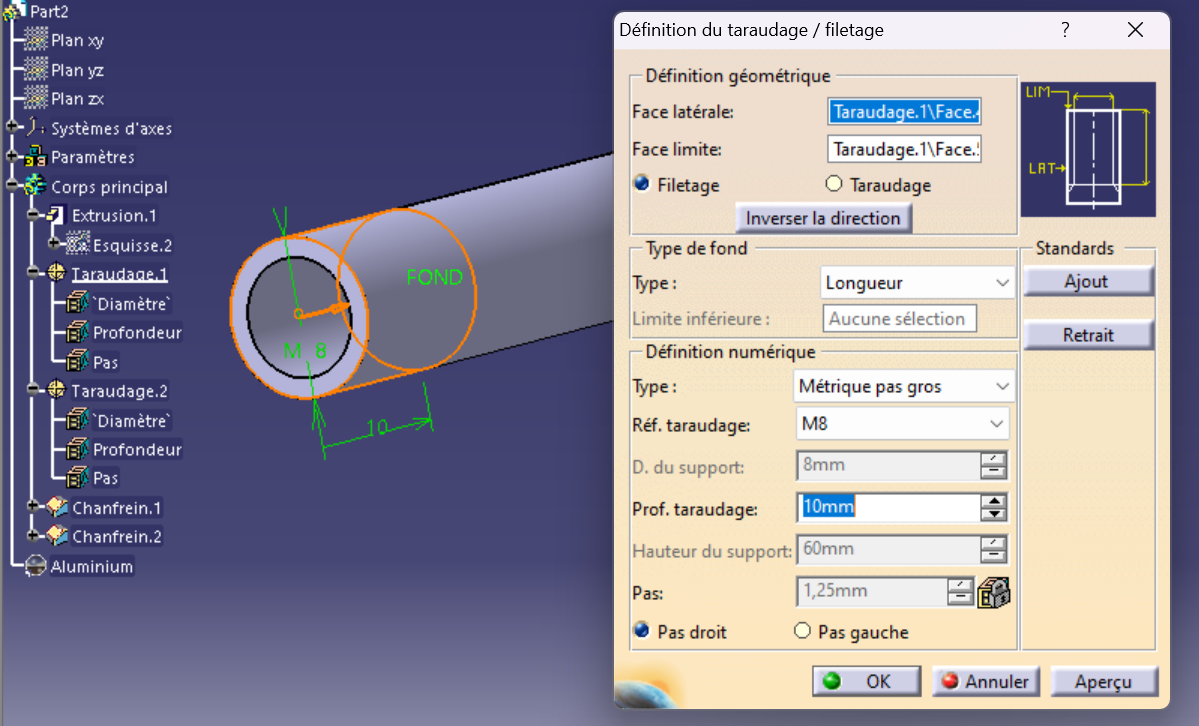
\includegraphics[width=0.7\textwidth]{images/filetage_tube_m8.png}
        \caption{Création du filetage M8 aux extrémités du tube de liaison}
        \label{fig:filetage_tube}
    \end{figure}
    
    \item \textbf{Finalisation du tube de liaison}:
    \begin{itemize}
        \item Le tube de liaison est maintenant terminé, prêt à être intégré dans l'assemblage
        \item Caractéristiques principales de cette pièce:
        \begin{itemize}
            \item Structure tubulaire en aluminium offrant un excellent rapport résistance/poids
            \item Diamètre extérieur de 10mm et intérieur de 8mm (épaisseur de paroi de 1mm)
            \item Longueur totale de 60mm permettant l'écartement optimal des moteurs
            \item Filetages M8 (pas 1,25mm) aux deux extrémités pour la connexion avec les autres pièces
            \item Passage interne pour les câbles électriques des moteurs
        \end{itemize}
        \item Finitions appliquées:
        \begin{itemize}
            \item Ajout de chanfreins de 0,5 mm aux extrémités du tube pour faciliter l'insertion et éviter les bavures
            \item Utilisation des fonctions Chanfrein.1 et Chanfrein.2 visible dans l'arborescence du modèle
            \item Cette finition améliore à la fois l'aspect esthétique et la sécurité lors de la manipulation
        \end{itemize}
        \item Cette conception minimaliste remplit parfaitement les objectifs d'allègement de la structure tout en maintenant la rigidité nécessaire pour un drone performant
    \end{itemize}
\end{enumerate}

\begin{figure}[H]
    \centering
    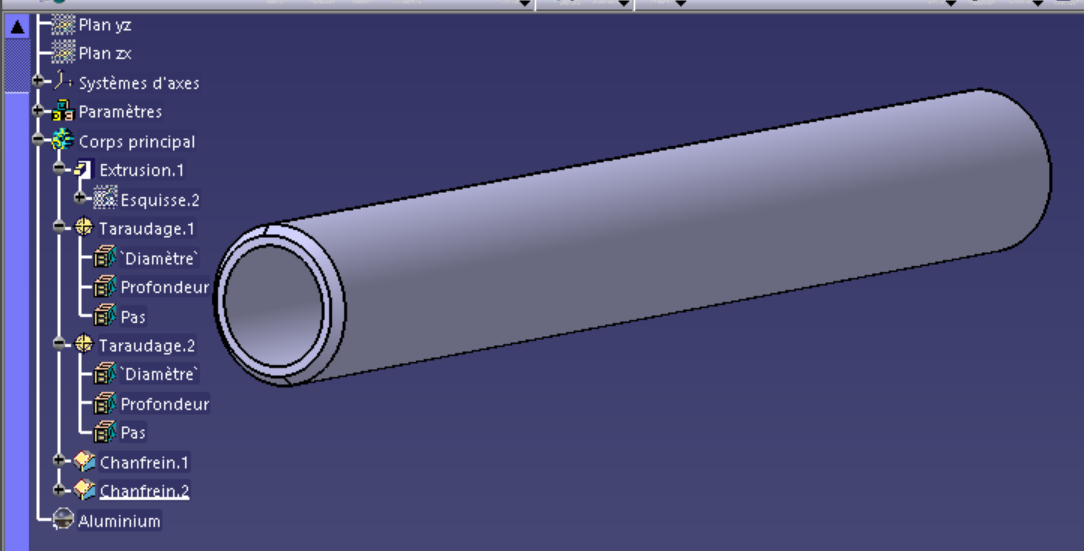
\includegraphics[width=0.7\textwidth]{images/tube_liaison_complet.png}
    \caption{Vue finale du tube de liaison avec l'arborescence complète (taraudages et chanfreins)}
    \label{fig:tube_liaison_arborescence}
\end{figure}

Cette pièce de liaison constitue un élément essentiel dans l'architecture du drone, permettant de relier le châssis central aux supports moteurs de façon légère et robuste. Sa conception tubulaire avec filetages intégrés illustre parfaitement l'approche d'optimisation mécanique nécessaire dans le domaine des drones, où chaque gramme économisé permet d'augmenter l'autonomie de vol.

\subsection{Modélisation des supports de moteur}
Pour modéliser les supports de moteur qui servent d'interface entre les bras et les moteurs, nous avons procédé comme suit:
\begin{enumerate}
    \item \textbf{Création d'une esquisse sur le plan supérieur du bras}:
    \begin{itemize}
        \item Dessin d'un cercle de diamètre 30mm centré sur l'extrémité du bras
        \item Application des contraintes de concentricité avec l'axe central du bras
    \end{itemize}
    \item \textbf{Opération de multi-extrusion}:
    \begin{itemize}
        \item Utilisation de la fonction multi-extrusion pour générer l'épaisseur du support
        \item Paramétrage de deux domaines d'extrusion : 2mm et 10mm
    \end{itemize}
    \begin{figure}[H]
        \centering
        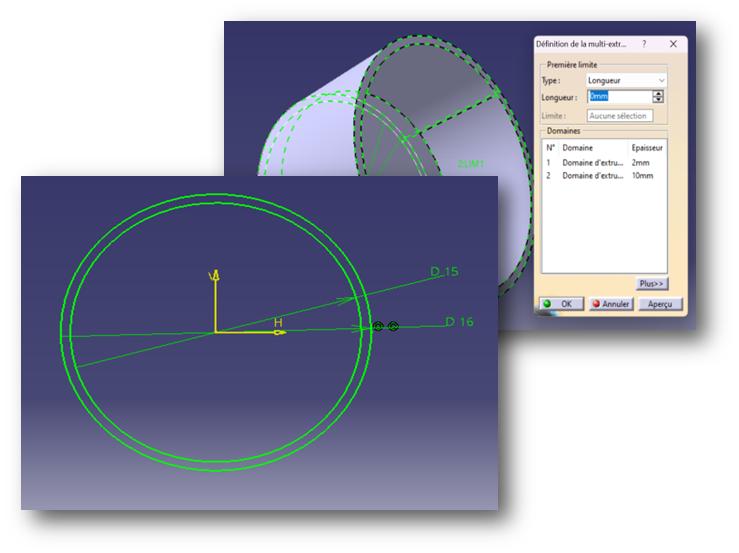
\includegraphics[width=0.7\textwidth]{images/multi_extrusion_tube.png}
        \caption{Opération de multi-extrusion sur l'esquisse du support de moteur}
        \label{fig:multi_extrusion_tube}
    \end{figure}
    
    \item \textbf{Création de l'évidement central}:
    \begin{itemize}
        \item Création d'un plan décalé à la distance souhaitée depuis la base du support
        \item Réalisation d'une esquisse circulaire sur ce plan pour définir l'évidement (diamètre intérieur)
        \item Utilisation de l'opération d'extrusion "jusqu'au suivant" pour percer le support selon l'esquisse
    \end{itemize}
    \begin{figure}[H]
        \centering
        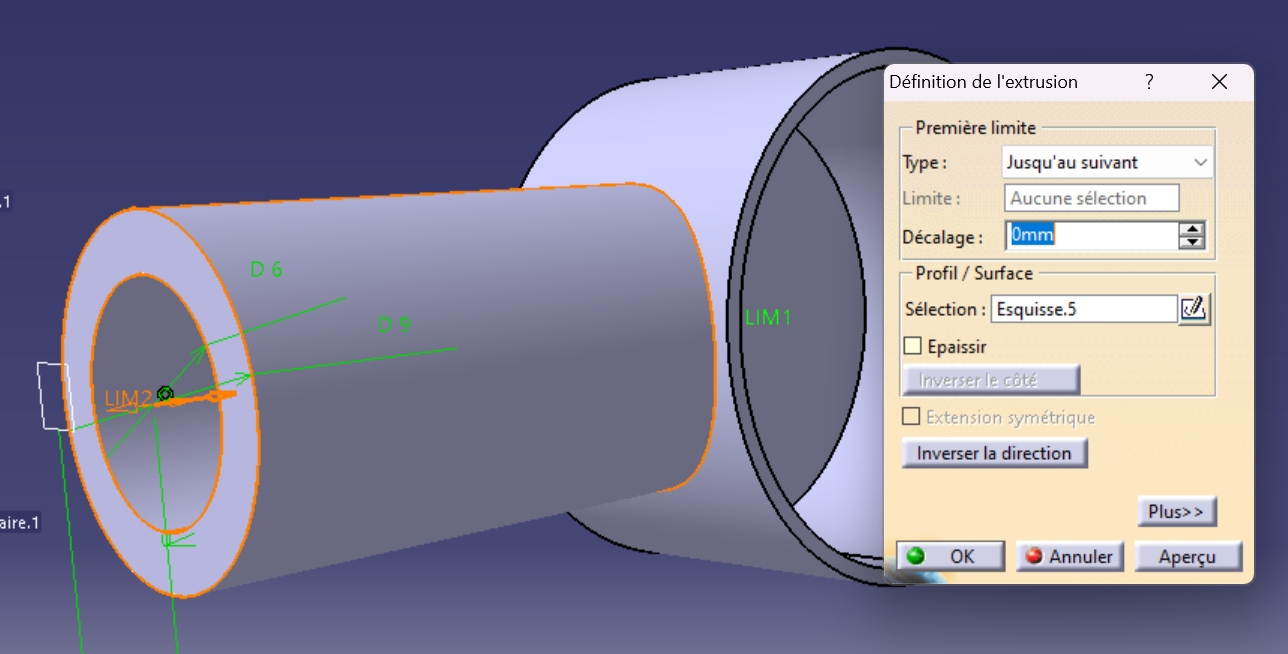
\includegraphics[width=0.7\textwidth]{images/extrusion_evidement_support.png}
        \caption{Extrusion de l'évidement central du support de moteur à partir d'un plan décalé}
        \label{fig:extrusion_evidement_support}
    \end{figure}
    
    \item \textbf{Création des points de fixation}:
    \begin{itemize}
        \item Création d'une poche (Pocket) pour préparer la zone d'implantation des trous de fixation
        \item Réalisation d'une extrusion locale pour donner l'épaisseur nécessaire autour des futurs trous
        \item Perçage d'un premier trou de fixation (Trou.2) selon la norme de montage des moteurs brushless
        \item Application d'une répétition circulaire (Circular Pattern) du trou autour de l'axe central
        \item Paramètres : 4 instances, espacement angulaire 90°, angle total 360°, référence axiale : Repère absolu/Axe
    \end{itemize}
    \begin{figure}[H]
        \centering
        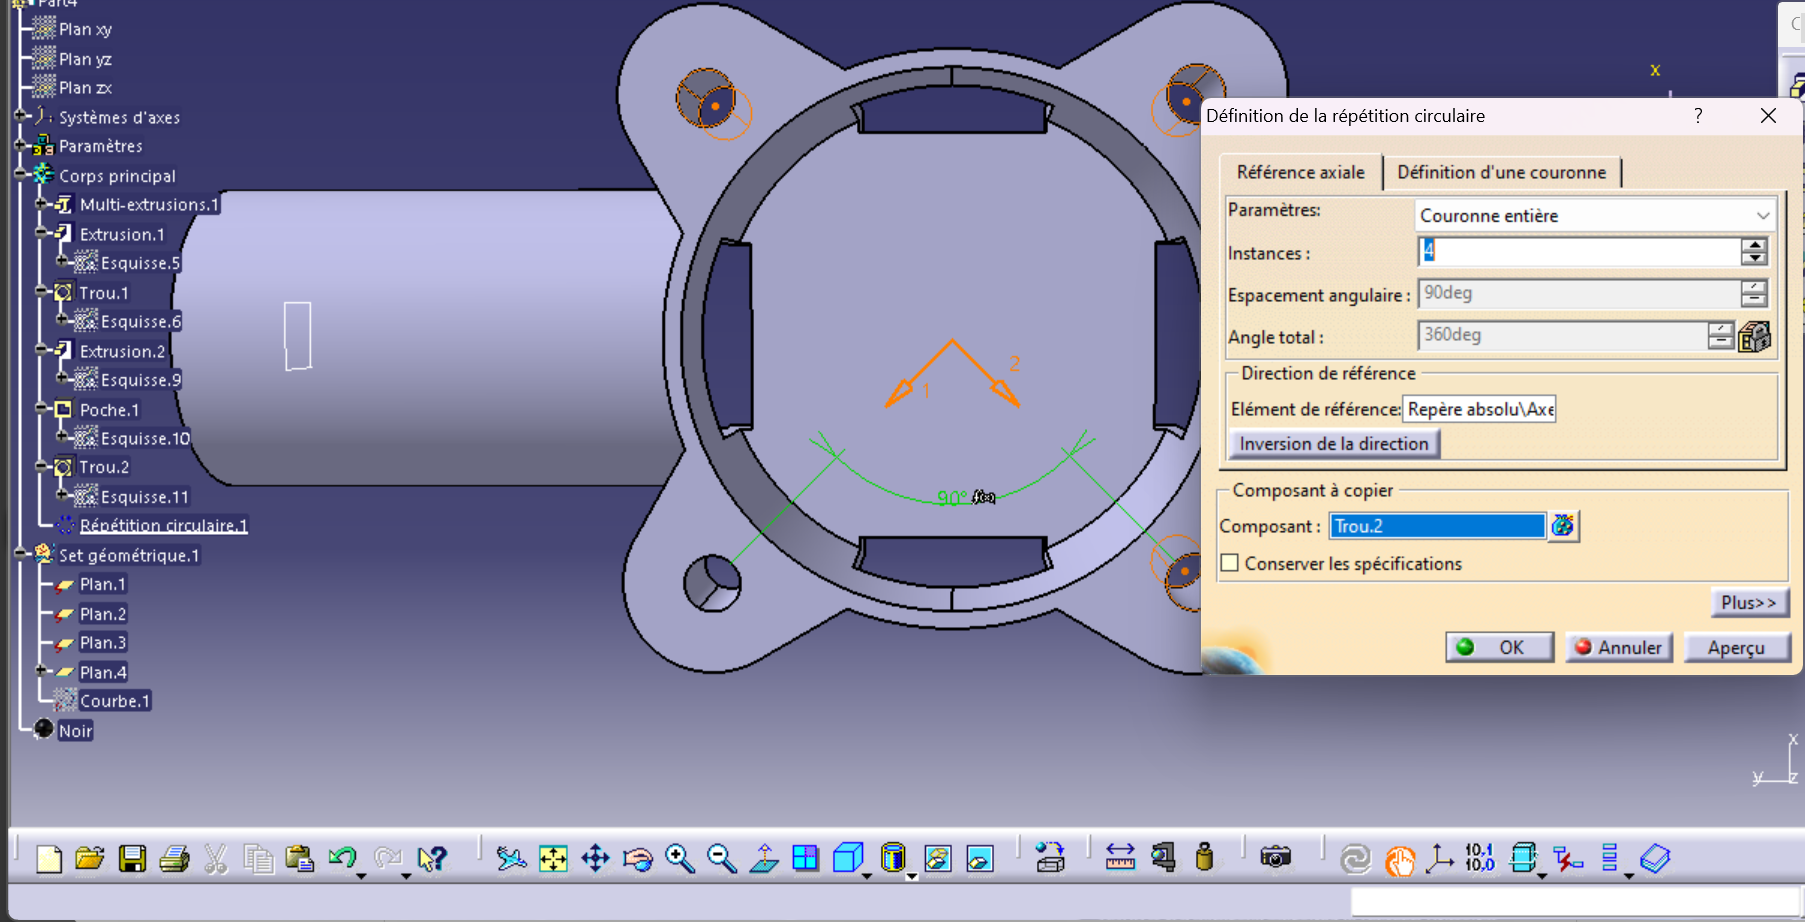
\includegraphics[width=0.9\textwidth]{images/repetition_circulaire_trous_support.png}
        \caption{Répétition circulaire des trous de fixation sur le support de moteur (CATIA V5)}
        \label{fig:repetition_circulaire_trous_support}
    \end{figure}
    
    \item \textbf{Finitions}:
    \begin{itemize}
        \item Application de congés de rayon 1mm sur toutes les arêtes exposées
        \item Chanfreins de 0.5x45° autour des trous de fixation
    \end{itemize}
\end{enumerate}

\begin{figure}[H]
    \centering
    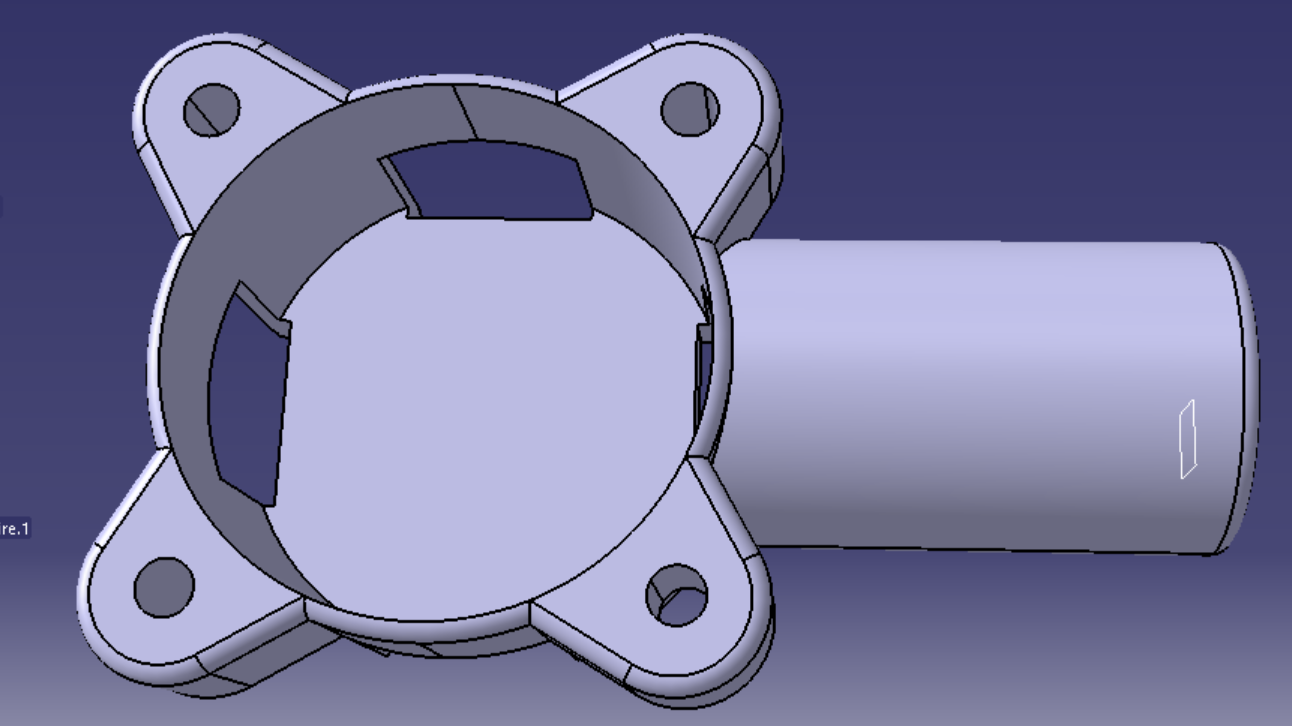
\includegraphics[width=0.7\textwidth]{images/support_moteur_final.png}
    \caption{Vue 3D du support de moteur finalisé avec tous les détails}
    \label{fig:support_moteur}
\end{figure}

\subsection{Modélisation des hélices}
Pour modéliser les hélices de couleur bleue, nous avons procédé comme suit :
\begin{enumerate}
    \item \textbf{Création de la géométrie de base de l'hélice} :
    \begin{itemize}
        \item Création d'un cercle représentant le moyeu central de l'hélice.
        \item Ajout d'un point sur le cercle pour définir le départ de la pale.
        \item Utilisation de l'atelier Generative Shape Design pour générer une courbe hélicoïdale à partir du point créé sur le cercle.
        \item Création d'un second cercle, concentrique au premier, représentant la longueur maximale de la pale.
        \item Réalisation d'une extrusion surfacique de ce cercle pour obtenir un cylindre de référence.
        \item Projection de la première hélice sur la surface du cylindre pour obtenir deux courbes hélicoïdales :
    \begin{itemize}
            \item Une sur le cylindre intérieur (rayon min)
            \item Une sur le cylindre extérieur (rayon max)
    \end{itemize}
        \item Création de courbes de liaison entre les deux hélices pour définir le profil de la pale.
        \item Utilisation de la fonction "remplissage surfacique" pour générer une surface entre les deux courbes hélicoïdales.
        \item Application d'une opération de découpe pour obtenir la forme définitive de la pale d'hélice.
    \end{itemize}
    \begin{figure}[H]
        \centering
        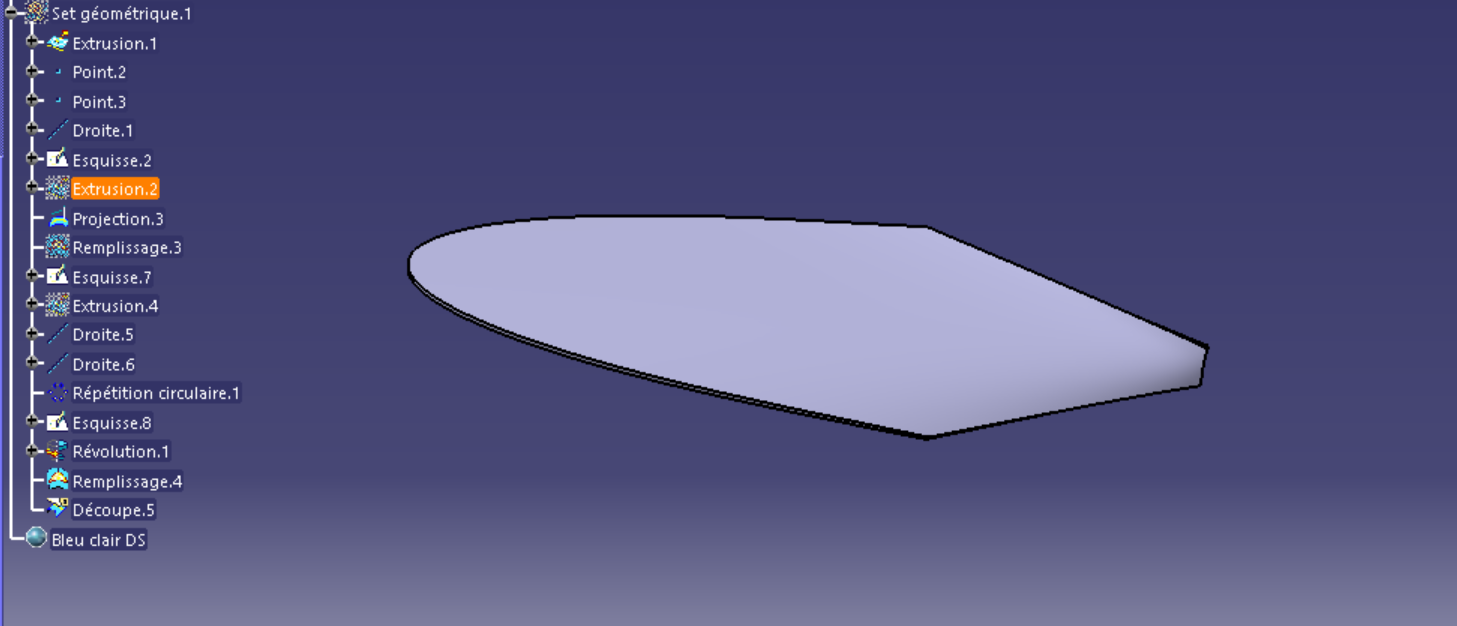
\includegraphics[width=0.8\textwidth]{images/esquisse_extrusion_helice.png}
        \caption{Étapes de création de la surface de l'hélice à partir de l'esquisse et de l'extrusion surfacique}
        \label{fig:esquisse_extrusion_helice}
    \end{figure}
    
    \item \textbf{Finitions}:
    \begin{itemize}
        \item Application d'un congé sur les bords d'attaque et de fuite des pales
        \item Réalisation d'un trou central pour la fixation sur l'axe du moteur
    \end{itemize}
    
    \item \textbf{Duplication}:
    \begin{itemize}
        \item Utilisation de la fonction répétition circulaire pour répliquer les hélices de deusieme côté
    \end{itemize}
    
    \item \textbf{Application du matériau}:
    \begin{itemize}
        \item Application d'un matériau plastique léger
        \item Attribution de la couleur bleue (propriété visible sur l'image)
    \end{itemize}
\end{enumerate}

\begin{figure}[H]
    \centering
    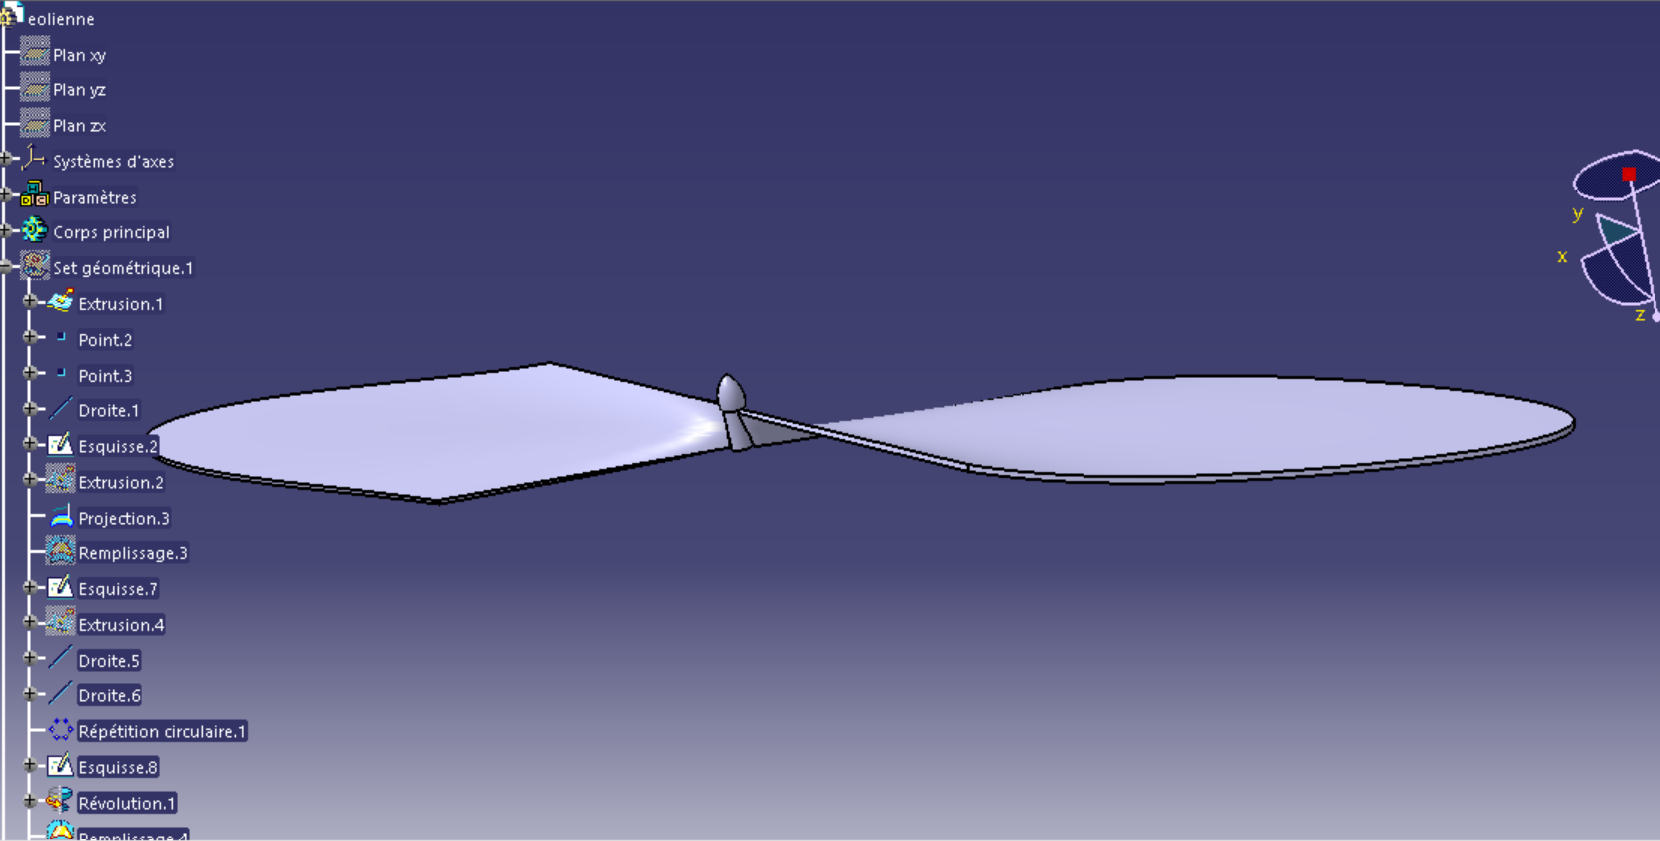
\includegraphics[width=0.7\textwidth]{images/helice_drone.png}
    \caption{Extrait du dessin de définition d'une hélice}
    \label{fig:dessin_helice}
\end{figure}

\subsection{Modélisation du support d'attache}
Pour modéliser le support d'attache, nous avons procédé comme suit :
\begin{enumerate}
    \item \textbf{Définition de la géométrie du guide}
    \begin{itemize}
        \item Définition des coordonnées de chaque point clé du support dans l'espace 3D.
        \item Utilisation de la fonction "Spline" pour créer une courbe passant par tous ces points, formant ainsi le guide du support.
        \item Application de contraintes de tangence pour garantir la continuité et la douceur de la courbe.
    \end{itemize}
    \item \textbf{Création du profil et génération du volume}
    \begin{itemize}
        \item Tracé d'un profil circulaire (section du tube) dans une esquisse positionnée à l'extrémité du guide.
        \item Utilisation de l'opération "Nervure" (Rib) pour balayer le profil circulaire le long du guide spline, générant ainsi la forme tubulaire du support d'attache.
    \end{itemize}
    \item \textbf{Opération de coque (Shell)}
    \begin{itemize}
        \item Application de l'opération "Coque" pour évider l'intérieur du support, simulant ainsi la fabrication réelle par formage d'un tube.
    \end{itemize}
\end{enumerate}
\begin{figure}[H]
    \centering
    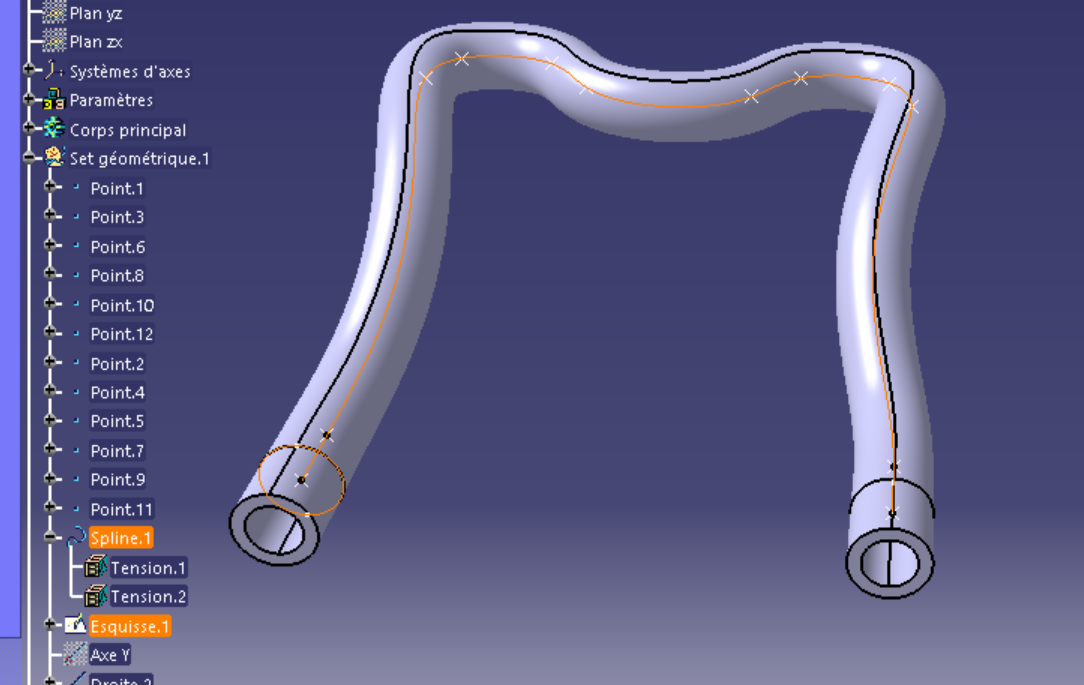
\includegraphics[width=0.8\textwidth]{images/support_attache_spline_nervure.png}
    \caption{Création du support d'attache par balayage d'un profil circulaire le long d'une courbe spline, puis évidement par opération de coque}
    \label{fig:support_attache_spline_nervure}
\end{figure}

\subsection{Modélisation du capot de protection électronique}
Le capot de protection électronique a été modélisé selon les étapes suivantes :
\begin{itemize}
    \item Multi-extrusion de la base du capot pour obtenir différentes épaisseurs selon les zones.
    \begin{figure}[H]
        \centering
        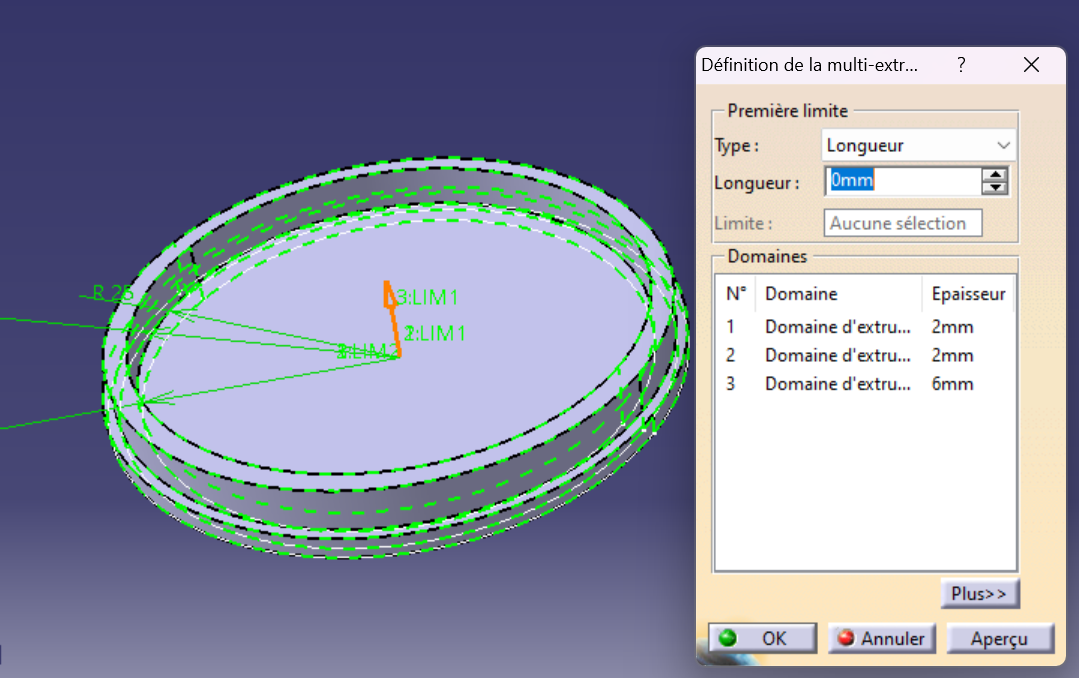
\includegraphics[width=0.7\textwidth]{images/multi_extrusion_capot.png}
        \caption{Multi-extrusion de la base du capot de protection électronique}
        \label{fig:multi_extrusion_capot}
    \end{figure}
    \item Ajout de nervures de renfort à l'aide de l'atelier Generative Shape Design pour rigidifier la structure.
    \begin{figure}[H]
        \centering
        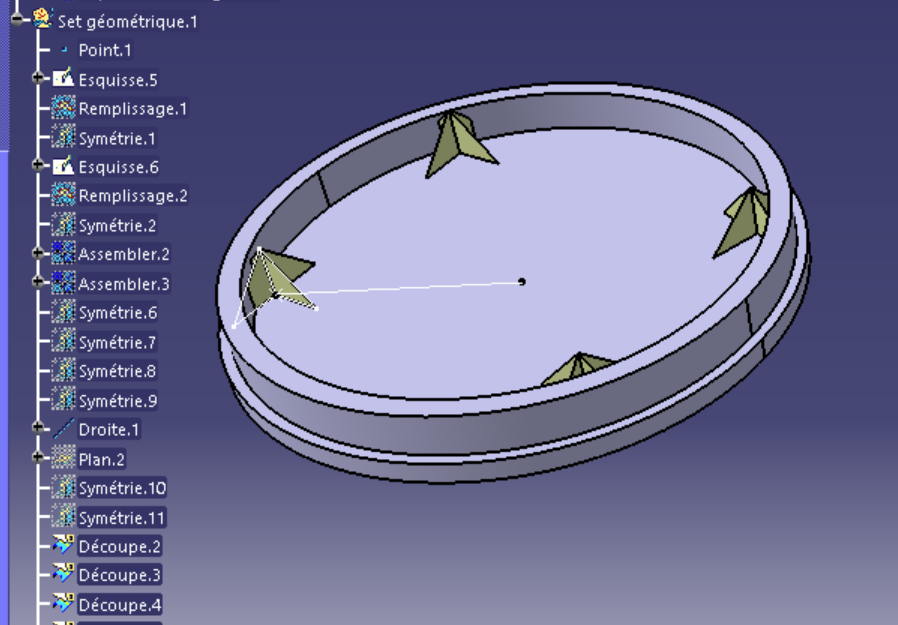
\includegraphics[width=0.7\textwidth]{images/nervures_capot.png}
        \caption{Ajout des nervures de renfort sur le capot}
        \label{fig:nervures_capot}
    \end{figure}
    \item Ajout de bossages (pousages) qui recevront par la suite les trous de fixation.
    \begin{figure}[H]
        \centering
        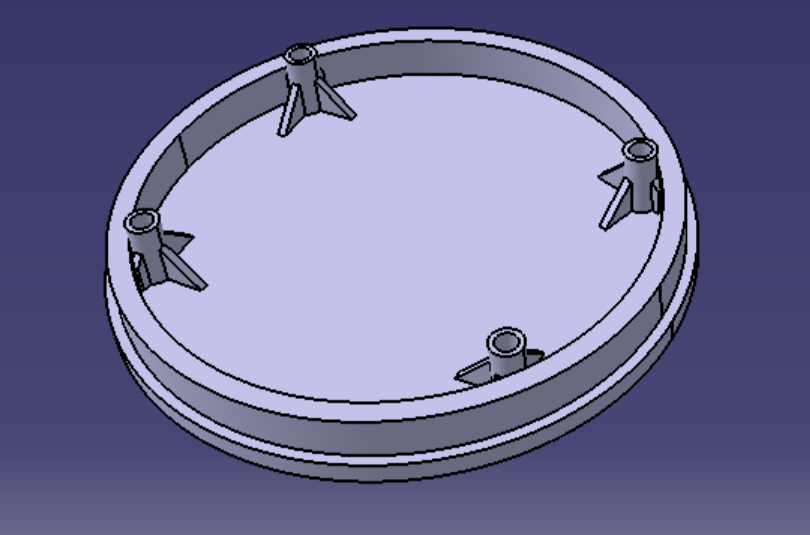
\includegraphics[width=0.7\textwidth]{images/bossages_trous_capot.png}
        \caption{Ajout des bossages et perçage des trous de fixation sur le capot}
        \label{fig:bossages_trous_capot}
    \end{figure}
    \item Réalisation des trous de fixation dans les bossages pour permettre l'assemblage du capot sur le châssis.
\end{itemize}

\subsection{Modélisation des éléments de fixation}
Les éléments de fixation utilisés dans ce projet sont des composants standards issus des catalogues ISO. Ils ont été importés ou modélisés selon les normes en vigueur, ce qui garantit leur compatibilité et leur disponibilité industrielle.

\begin{itemize}
    \item 4 vis pour la fixation de chaque moteur sur son support (exemple : ISO 1207 M2x5, tête fendue)
    \begin{figure}[H]
        \centering
        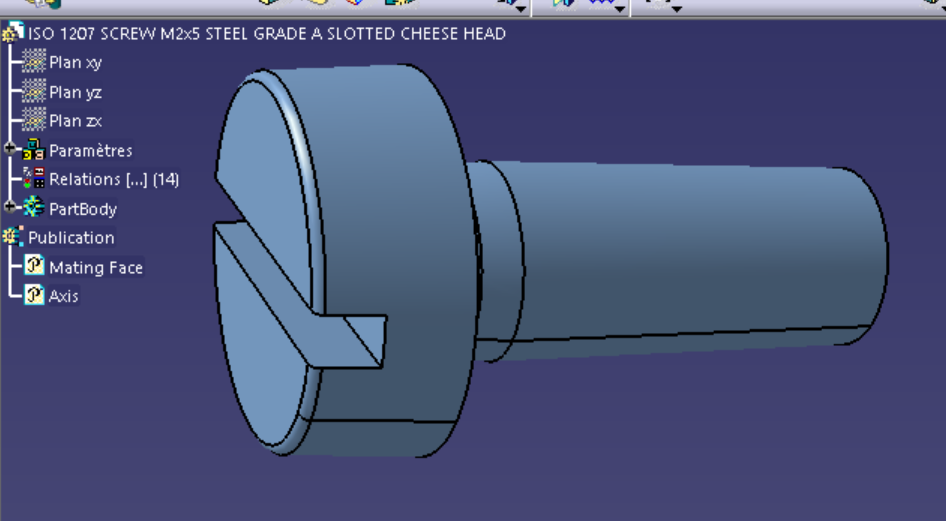
\includegraphics[width=0.5\textwidth]{images/vis_iso_m2x5.png}
        \caption{Vis standard ISO 1207 M2x5 pour la fixation des moteurs}
        \label{fig:vis_iso_m2x5}
    \end{figure}
    \item 4 vis pour la fixation du capot de protection sur le bâti central (exemple : ISO 1207 M1.6x16, tête fendue)
    \begin{figure}[H]
        \centering
        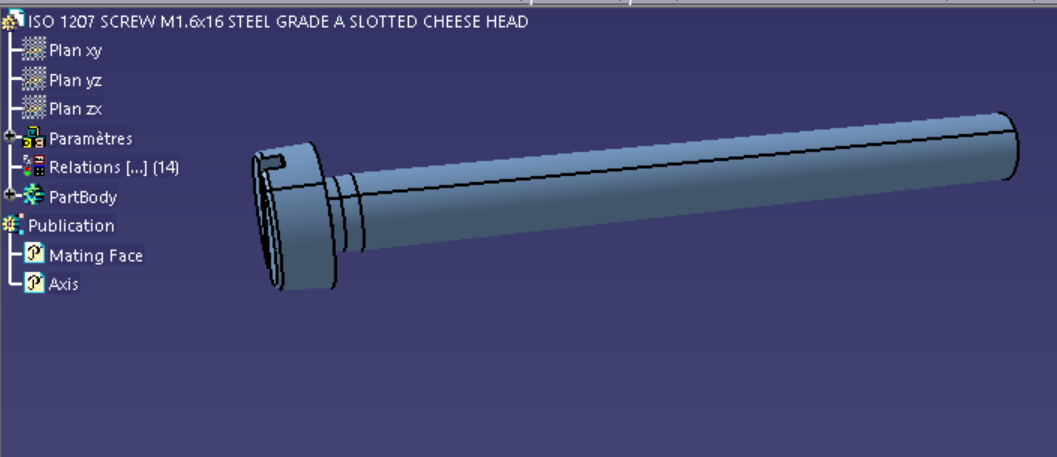
\includegraphics[width=0.7\textwidth]{images/vis_iso_m1_6x16.png}
        \caption{Vis standard ISO 1207 M1.6x16 pour la fixation du capot}
        \label{fig:vis_iso_m1_6x16}
    \end{figure}
\end{itemize}

L'utilisation de ces éléments standards permet d'assurer la fiabilité de l'assemblage, la facilité de maintenance et le remplacement rapide en cas de besoin.

\subsection{Modélisation et choix du moteur}
Pour l'entraînement du drone, quatre moteurs identiques ont été sélectionnés. Ces moteurs proviennent d'un catalogue industriel (exemple : https://www.traceparts.com/fr/) afin de garantir la fiabilité, la disponibilité et la conformité aux normes.

\begin{itemize}
    \item Les caractéristiques principales du moteur choisi sont les suivantes :
    \begin{itemize}
        \item Diamètre d'alésage : 35 mm
        \item Diamètre extérieur : 72 mm
        \item Largeur : 17 mm
        \item Angle de contact : 25°
        \item Capacité de charge dynamique : 35,5 kN
        \item Capacité de charge statique : 23,2 kN
        \item Vitesse de référence : 12 000 tr/min
        \item Vitesse limite : 19 000 tr/min
        \item Classe de performance : SKF Explorer
    \end{itemize}
    \begin{figure}[H]
        \centering
        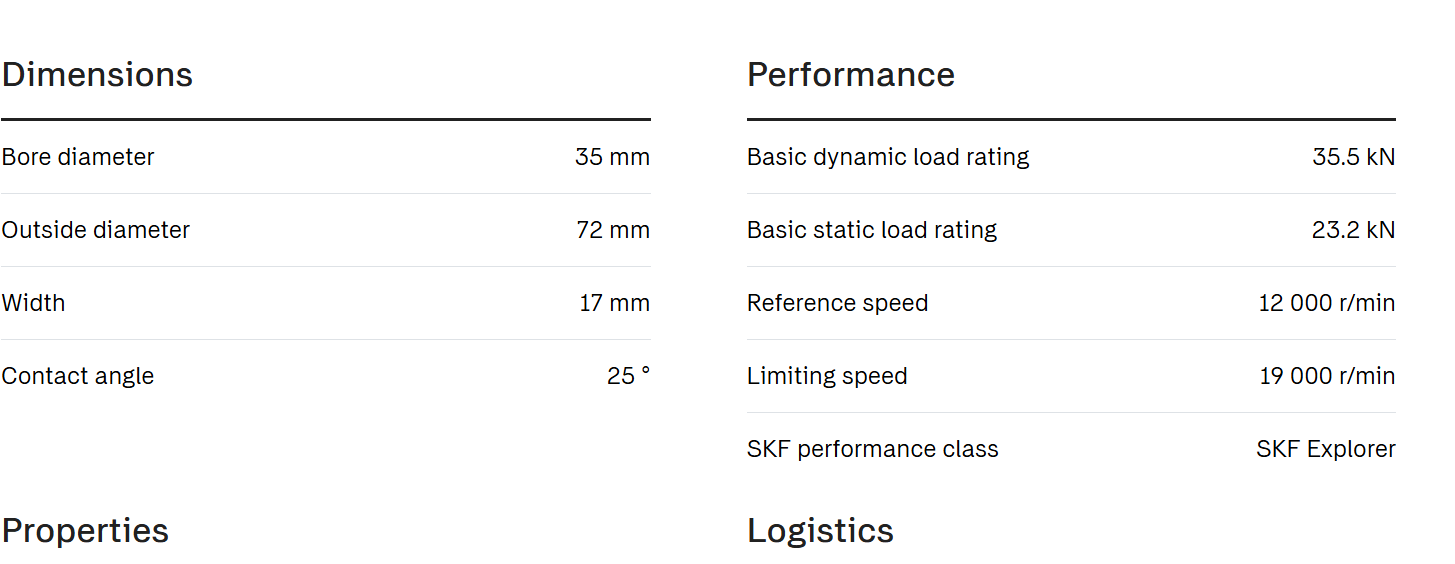
\includegraphics[width=0.8\textwidth]{images/moteur_caracteristiques.png}
        \caption{Caractéristiques techniques du moteur sélectionné (extrait de catalogue)}
        \label{fig:moteur_caracteristiques}
    \end{figure}
    \item Le modèle 3D du moteur a été importé ou modélisé à partir des données du fournisseur pour garantir la compatibilité avec le support moteur et l'ensemble du drone.
    \begin{figure}[H]
        \centering
        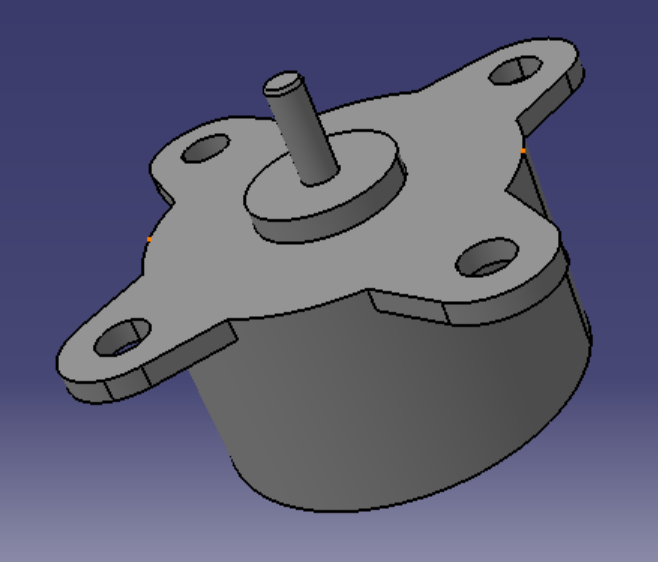
\includegraphics[width=0.5\textwidth]{images/moteur_modele.png}
        \caption{Modélisation 3D du moteur utilisé pour l'entraînement du drone}
        \label{fig:moteur_modele}
    \end{figure}
\end{itemize}

L'utilisation de moteurs standards issus de catalogue permet d'assurer la robustesse, la maintenance aisée et la disponibilité des pièces de rechange.

\chapter{Assemblage}
\section{Structure de l'assemblage}
L'assemblage complet du drone quadrirotor est composé des éléments suivants :
    \begin{itemize}
        \item Châssis central (corps principal)
        \item Bras de support (4 pièces)
    \item Support de moteur (4 pièces)
        \item Capot de protection électronique
        \item Moteurs brushless (4 pièces)
        \item Hélices (4 pièces)
    \item Support d'attache (2 pièces)
        \item Système de fixation pour accessoires
\end{itemize}

\begin{figure}[H]
    \centering
    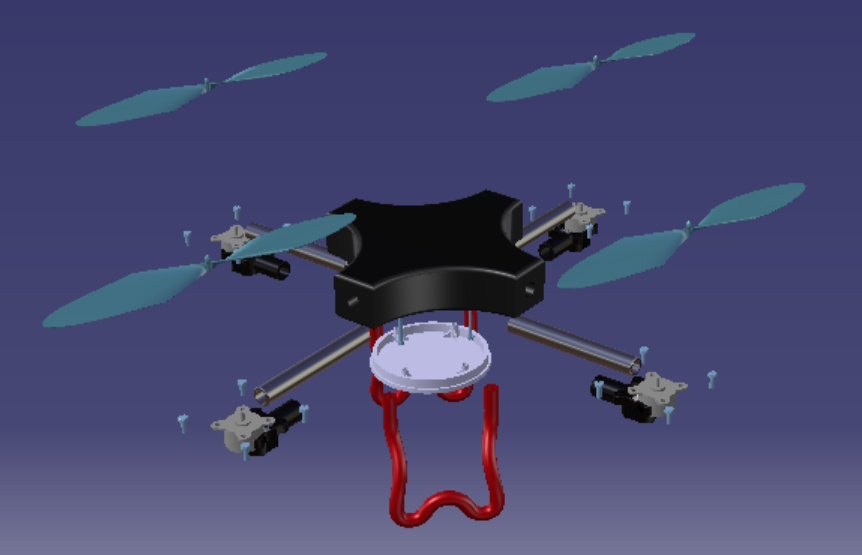
\includegraphics[width=0.8\textwidth]{images/vue_eclatee_drone.png}
    \caption{Vue éclatée du drone quadrirotor réalisée sous CATIA V5}
    \label{fig:vue_eclatee_drone}
\end{figure}

\section{Contraintes d'assemblage}
Pour réaliser l'assemblage du drone, nous avons utilisé les contraintes suivantes:

\begin{itemize}
    \item \textbf{Contraintes de positionnement du châssis}:
    \begin{itemize}
        \item Fixation du châssis central comme pièce de référence
        \item Positionnement dans le plan XY avec l'axe Z représentant la hauteur
    \end{itemize}
    
    \item \textbf{Contraintes des bras de support}:
    \begin{itemize}
        \item Contrainte de coïncidence entre les trous de fixation des bras et ceux du châssis
        \item Contrainte de contact entre la face inférieure des bras et la face supérieure du châssis
        \item Contrainte angulaire pour l'espacement régulier à 90° entre chaque bras
    \end{itemize}
    
    \item \textbf{Contraintes des moteurs}:
    \begin{itemize}
        \item Contrainte de coïncidence entre l'axe du moteur et l'axe du trou dans le support de moteur
        \item Contrainte de contact entre la base du moteur et la face du support moteur
        \item Contrainte angulaire pour l'orientation correcte des points de fixation
    \end{itemize}
    
    \item \textbf{Contraintes des supports de moteur}:
    \begin{itemize}
        \item Contrainte de coïncidence entre l'axe du support et l'axe de l'extrémité du bras
        \item Contrainte de contact entre la face inférieure du support et la face supérieure du bras
        \item Contrainte d'alignement des trous de fixation entre le support et le bras
    \end{itemize}
    
    \item \textbf{Contraintes des hélices}:
    \begin{itemize}
        \item Contrainte de coïncidence entre l'axe de l'hélice et l'axe du moteur
        \item Contrainte de distance pour le positionnement en hauteur
        \item Contrainte d'orientation pour les sens de rotation opposés (horaire/anti-horaire)
    \end{itemize}
    
    \item \textbf{Contraintes du support d'attache}:
    \begin{itemize}
        \item Contrainte de coïncidence entre les trous de fixation du support et ceux du châssis
        \item Contrainte de contact entre la face supérieure du support et la face inférieure du châssis
        \item Contrainte de symétrie par rapport au plan central
    \end{itemize}
\end{itemize}

\begin{figure}[H]
    \centering
    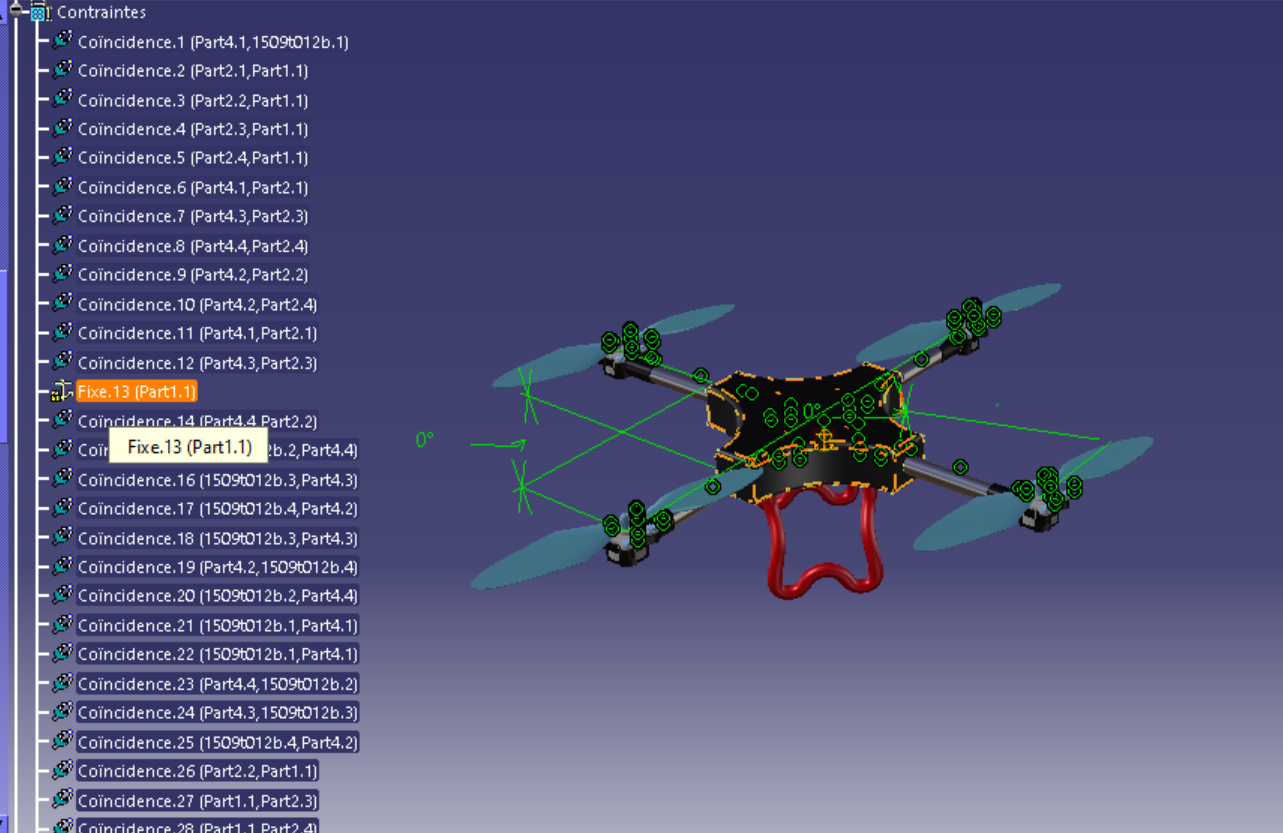
\includegraphics[width=0.9\textwidth]{images/contraintes_assemblage_drone.png}
    \caption{Vue des contraintes d'assemblage appliquées dans CATIA V5 pour le drone quadrirotor}
    \label{fig:contraintes_assemblage_drone}
\end{figure}

\section{Rendu photoréaliste}
Le drone quadrirotor finalisé est présenté ci-dessous dans un rendu photoréaliste. Cette visualisation permet d'apprécier l'assemblage complet des différents composants, notamment la disposition symétrique des quatre bras de support, les moteurs et leurs hélices respectives, ainsi que le châssis central qui assure la rigidité de l'ensemble.

\begin{figure}[H]
    \centering
    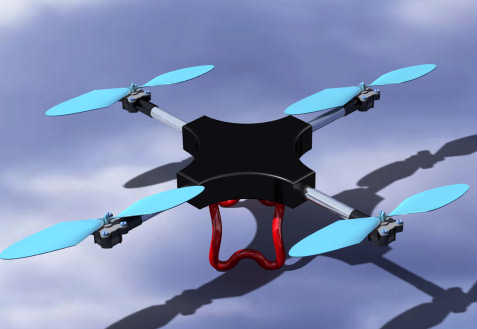
\includegraphics[width=0.8\textwidth]{images/drone_apercu.png}
    \caption{Rendu photoréaliste du drone quadrirotor finalisé}
    \label{fig:rendu_final}
\end{figure}

\chapter{Dessin de définition}
\section{Cotation fonctionnelle}
Pour chaque pièce du drone, nous avons réalisé un dessin de définition avec une cotation fonctionnelle complète:

\begin{figure}[H]
    \centering
    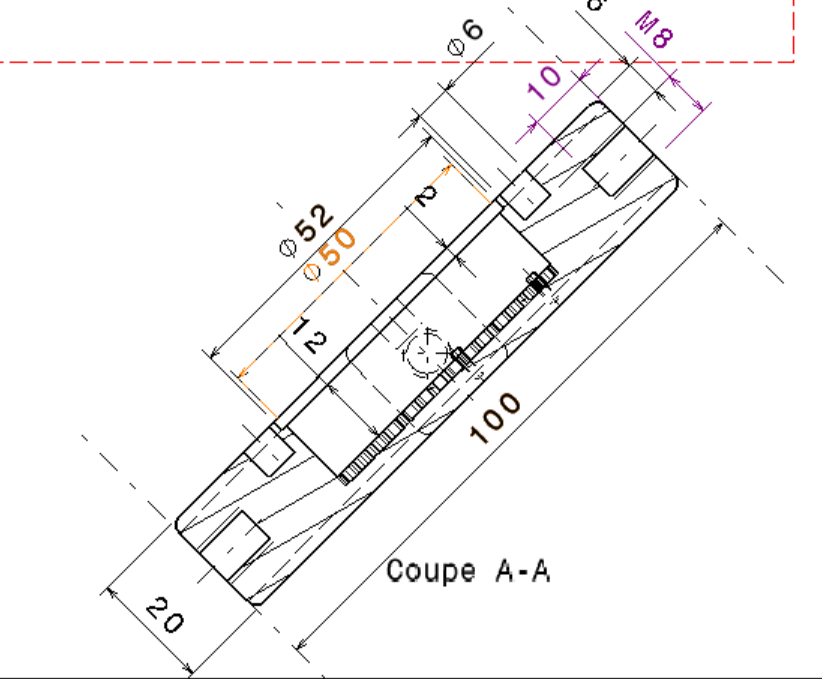
\includegraphics[width=0.8\textwidth]{images/exemple_cotation_fonctionnelle.png}
    \caption{Exemple de cotation fonctionnelle pour une pièce du drone}
    \label{fig:exemple_cotation_fonctionnelle}
\end{figure}

\section{Mise en plan}
La mise en plan a été réalisée selon les normes ISO, avec:

\begin{itemize}
    \item \textbf{Cartouche normalisé} contenant:
    \begin{itemize}
        \item Nom de la pièce
        \item Échelle du dessin
        \item Matériau
        \item Référence
        \item Date de création
        \item Nom du concepteur
    \end{itemize}
    
    \begin{figure}[H]
        \centering
        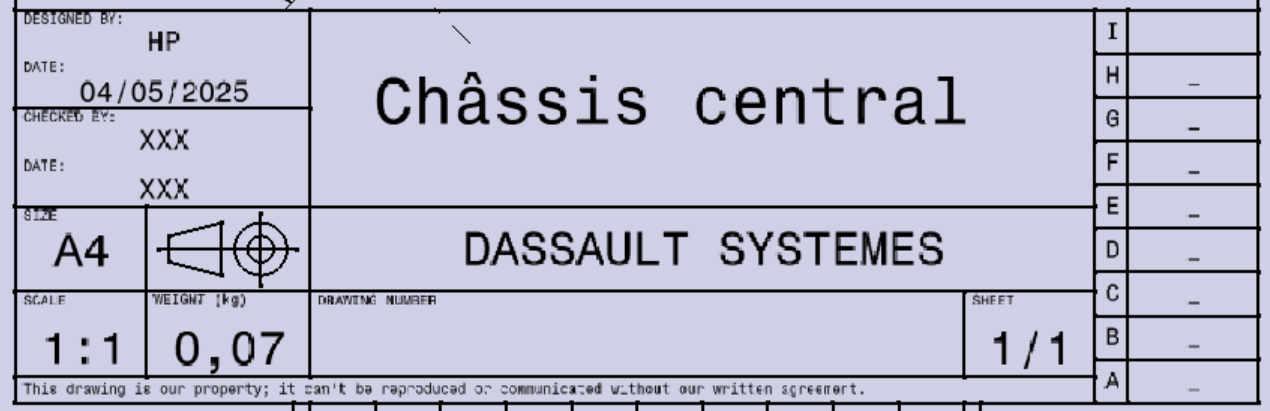
\includegraphics[width=0.8\textwidth]{images/mise_en_plan_drone.png}
        \caption{Mise en plan du drone quadrirotor}
        \label{fig:mise_en_plan_drone}
    \end{figure}
    
    \item \textbf{Vues principales et coupes}:
    \begin{itemize}
        \item Vue de face, dessus et profil pour chaque pièce
        \item Coupes aux endroits stratégiques pour visualiser les détails internes
        \item Vues en perspective pour une meilleure compréhension
    \end{itemize}
    
    \item \textbf{Échelles adaptées}:
    \begin{itemize}
        \item Vue d'ensemble du châssis: 1:2
        \item Détails des fixations: 2:1
        \item Profil des hélices: 1:1
        \item Vue d'ensemble du drone: 1:5
    \end{itemize}
\end{itemize}

\subsection{Exemple: Dessin de définition du châssis central}

Le dessin ci-dessous présente la mise en plan détaillée du châssis central du drone. On y retrouve la vue de dessus, les coupes principales (A-A et B-B), ainsi que toutes les cotes fonctionnelles nécessaires à la fabrication et à l'assemblage de la pièce. Les dimensions critiques, telles que le diamètre extérieur, l'emplacement des perçages filetés M8, les rayons de courbure et l'épaisseur des parois, sont clairement indiquées. Ce plan respecte les normes de dessin industriel et intègre un cartouche complet précisant le nom de la pièce, l'échelle, la masse, la date, le concepteur et la société. Ce type de document est indispensable pour garantir la conformité de la pièce lors de la production.

\begin{figure}[H]
    \centering
    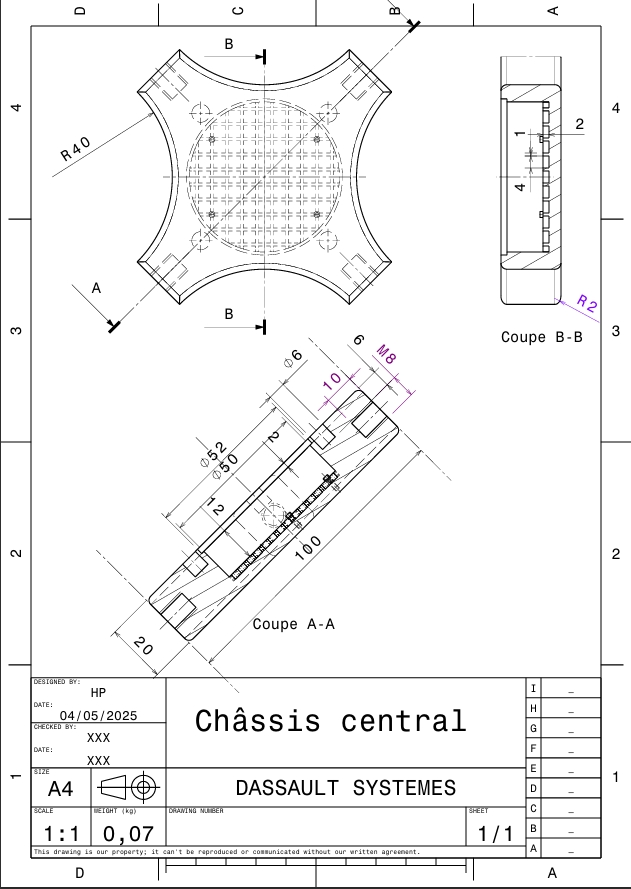
\includegraphics[width=0.8\textwidth]{images/chassis_central_plan.png}
    \caption{Dessin de définition du châssis central du drone quadrirotor}
    \label{fig:chassis_central_plan}
\end{figure}

Les dessins de définition complets de toutes les pièces, y compris les hélices, sont disponibles en annexe à la fin de ce rapport.

\chapter{Dessin d'ensemble}
\section{Nomenclature}
Le dessin d'ensemble du drone quadrirotor comprend une nomenclature complète avec :

\begin{itemize}
    \item \textbf{Numéro de repère} : Attribution séquentielle des numéros en commençant par le châssis
    \item \textbf{Désignation} : Nom précis de chaque composant
    \item \textbf{Matière} : Spécification des matériaux utilisés
    \item \textbf{Qté} : Nombre d'exemplaires
    \item \textbf{Obs.} : Remarques ou références
\end{itemize}

\begin{table}[H]
    \centering
    \small
    \caption{Nomenclature des composants du drone quadrirotor}
    \begin{tabular}{|c|l|c|c|l|}
        \hline
        \textbf{Rep.} & \textbf{Désignation} & \textbf{Matière} & \textbf{Qté} & \textbf{Obs.} \\
        \hline
        1 & Châssis central & PA6+30\%FV & 1 & Injecté, noir \\
        2 & Bras support & Alu 6061-T6 & 4 & Tube Ø10x8, 180mm \\
        3 & Support moteur & PA6+30\%FV & 4 & Impr. 3D/injecté \\
        4 & Moteur brushless & MT2212-920KV & 4 & Ø27.9mm, 55g \\
        5 & Hélice & ABS & 4 & 120mm, CW/CCW \\
        6 & Support attache & TPU & 2 & Impr. 3D, rouge \\
        7 & Capot protection & PC & 1 & Transparent \\
        8 & Vis moteur & Inox M2x8 & 16 & Tête cyl. \\
        9 & Vis support & Inox M3x15 & 4 & Tête cyl. \\
        \hline
    \end{tabular}
    \label{tab:nomenclature}
\end{table}

\section{Représentation et cotation d'encombrement}

La figure ci-dessous présente une vue d'ensemble du drone quadrirotor, illustrant la disposition des principaux composants et les dimensions d'encombrement. Ce dessin permet de visualiser l'architecture générale du système.

Le dessin d'ensemble comprend les cotes d'encombrement principales suivantes:
    \begin{itemize}
    \item Dimensions hors-tout: 300 × 300 × 120 mm (largeur × longueur × hauteur)
    \item Diamètre des hélices: 120 mm
    \item Hauteur du châssis: 20 mm
    \item Distance entre axes des moteurs opposés: 224 mm
\end{itemize}

\begin{figure}[H]
    \centering
    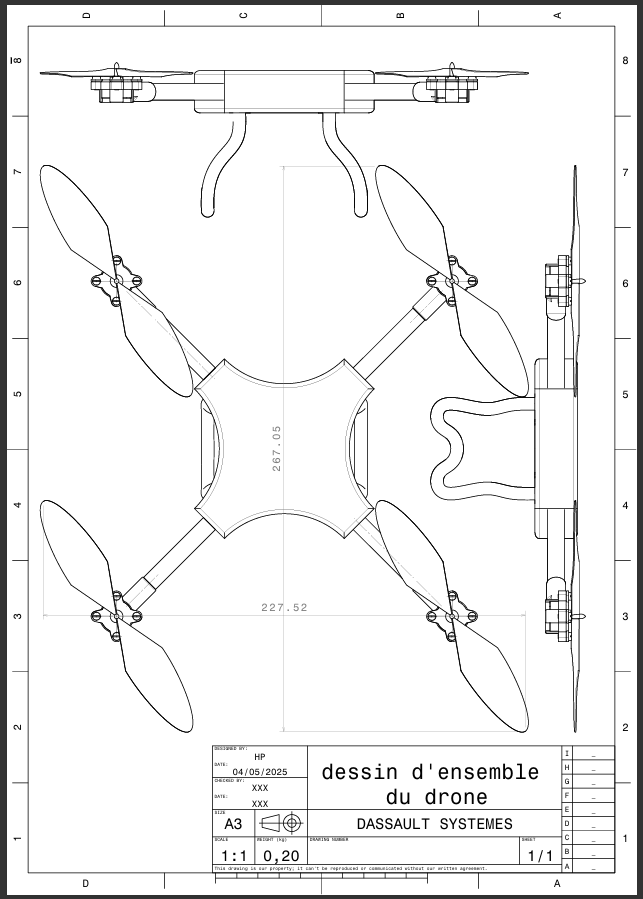
\includegraphics[width=0.8\textwidth]{images/dessin_ensemble_drone.png}
    \caption{Vue d'ensemble du drone quadrirotor (extrait du dessin d'ensemble)}
    \label{fig:dessin_ensemble_drone}
\end{figure}

Le dessin d'ensemble complet, avec toutes les vues et les détails cotés, est disponible en annexe à la fin de ce rapport.

\chapter{Analyse critique et conclusion}
\section{Conclusion}

Ce projet de conception d'un drone quadrirotor sur CATIA V5 nous a permis de développer nos compétences en conception assistée par ordinateur, notamment :

\begin{itemize}
    \item La maîtrise des fonctions avancées de modélisation 3D de CATIA V5 (extrusion, révolution, balayage, lissage)
    \item La compréhension des contraintes d'assemblage et leur application pratique
    \item L'utilisation des fonctions de mise en plan avec cotation fonctionnelle
    \item L'approche méthodique d'un projet complet, de la conception des pièces individuelles à l'assemblage final
\end{itemize}

Cette expérience nous a également sensibilisés à l'importance de l'optimisation mécanique, de la gestion des interférences et des contraintes liées à la fabrication. La réalisation de ce drone quadrirotor représente une application concrète des compétences d'ingénierie mécanique acquises durant notre formation.

Les défis rencontrés et surmontés durant ce projet constituent une préparation précieuse pour nos futures missions professionnelles, où nous serons amenés à concevoir des produits complexes en respectant des contraintes multiples.

\end{document} 